\chapter{Função do primeiro grau}

\section{Introdução}

A ideia de descrever o comportamento de uma grandeza relacionada com outra não é muito antiga. Os povos antigos, Árabes e Gregos não chegaram a investigar a velocidade. Foi com Galileo (1564-1642) ao estudar o movimento que o conceito de função começou a se configurar. Porém, não sem dificuldades. A geometria de Descartes (1637) já usava a representação gráfica de uma expressão algébrica, mas essa ideia só foi aceita na comunidade de matemáticos com os trabalhos de Euler (1707-1783) e da família dos Bernoillis, ao desenvolver o cálculo aplicado a problemas físicos. A definição atribuída a Euler diz que função \textit{é uma expressão analítica que representa a relação entre duas variáveis}. 

Um conceito de função, muito semelhante ao usado atualmente, foi introduzido por Dirichlet (1805-1859), motivado pela necessidade de uma definição mais restritiva que a de Euler, ao estudar o problema de convergência de séries, na época, aplicado à investigação de problemas de condução do calor, propostos por Fourier. A definição de Dirichlet é a seguinte: \textit{y é uma função de x, se para qualquer valor de x, existe uma regra que o associa a um único valor de y}. Em 1939, Bourbaki definiu função como \textit{regra de correspondência entre dois conjuntos e que isto era um subconjunto do produto cartesiano entre aqueles conjuntos}.

A definição de Euler é muito usada até hoje nas ciências, devido a sua simplicidade e eficiência para descrever a relação entre duas variáveis. De fato, muitas aplicações de funções na Física, Química e Economia requerem apenas uma expressão algébrica e uma representação gráfica.

Na base do desenvolvimento do Cálculo Diferencial e Integral está o conceito de função e daí sua importância, já que praticamente toda a ciência e a tecnologia moderna utilizam o Cálculo. Mas porque as funções são tão importantes para as ciências? Porque elas descrevem qualitativamente o comportamento de partes da realidade com precisão suficiente para que decisões possam ser tomadas. Saber o tempo de resfriamento de uma peça fundida é importante para decidir quando manuseá-la; saber o tempo em que a receita e a despesa de um empreendimento serão iguais, significa saber quando o lucro se inicia; o planejamento econômico de um reflorestamento depende da função de como as árvores crescem; a variação da concentração de um medicamento no organismo humano é fundamental para determinar a dose e o intervalo de ingestão; a deformação em vigas depende das cargas aplicadas e do material;... Todos esses e tantos outros fenômenos são expressos na forma de funções, cujo conhecimento básico vamos desenvolver neste capítulo.

\section{Definição de funções}

Analisemos o seguinte exemplo:

\begin{texemplo}
O preço de \textit{1 kg} de carne é \textit{R$\$$  15,00}. Determine uma fórmula para calcular qualquer o custo de quantidade de carne.

\textbf{Solução}: Vamos usar a ideia de variável. Seja \textit{x} a quantidade, em \textit{kg} e \textit{y} o custo da carne. Então

\textit{y = 15 $ \cdot $  x } \tab (2.1)
\end{texemplo}

é a expressão que dá o custo de carne para qualquer valor de \textit{x}. 

Se as massas são \textit{x = $ \{ $ 0, 0.5, 1, 2, 3$ \} $ ,} usando a Eq. (2.1) calculamos os correspondentes valores dos custos \textit{y =$ \{ $ 0, 7.5, 15, 30, 45$ \} $ }. Evidentemente, podemos calcular \textit{y} para qualquer \textit{x} real maior ou igual a zero.

\begin{texemplo}
Se \textit{x} é o lado de um quadrado, encontre uma expressão para a área.

\textbf{Solução}: Sabe-se que a área do quadrado é \textit{A = x\textsuperscript{2}}.  Para quadrados de lado \textit{x = $ \{ $ 0, 1, 2,3,4$ \} $ ,} usando a expressão da área temos os correspondentes valores de \textit{A=$ \{ $ 0,1,4,9,16$ \} $ }. Evidentemente, podemos calcular \textit{A} para qualquer  \textit{x} real maior ou igual a zero.
\end{texemplo}

\begin{caixa}
\begin{tdefinicao}
Sejam dois conjuntos \textit{X=$ \{ $ x\textsubscript{1}, x\textsubscript{2}, x\textsubscript{3}, x\textsubscript{4, }... x\textsubscript{n}$ \} $ }  e   \textit{Y=$ \{ $ y\textsubscript{1}, y\textsubscript{2}, y\textsubscript{3}, y\textsubscript{4, }..., y\textsubscript{n} $ \} $ }. Seja \textit{f  }uma regra matemática que associa os elementos de \textit{X} e \textit{Y}, formando um  conjunto de pares ordenados (\textit{x\textsubscript{i}, y\textsubscript{i}}) com \textit{i =1,2,3,4, ...,n. Y =f(x\textsubscript{i})} é uma função de \textit{X}, se para qualquer \textit{ x\textsubscript{i }, f}  associa um, e somente um valor de\textit{ y\textsubscript{i}}. 
\end{tdefinicao}
\end{caixa}

Nos pares ordenados (\textit{x,y}), os elementos do conjunto \textit{X} são chamados de \textit{abcissas} e os do conjunto \textit{Y} de \textit{ordenadas}.

\begin{figure}[H]
	\begin{Center}
		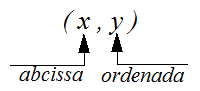
\includegraphics[width=2.08in,height=0.95in]{capitulos/funcao_do_primeiro_grau/media/image2.png}
	\end{Center}
\end{figure}

As expressões dos Exemplos 2.1 e 2.2 são funções de acordo com a Def. 2.1, pois para cada valor de \textit{x}, existe um e somente um \textit{y}. 

\begin{texemplo}
Represente a função do Exemplo 2.1 em um gráfico cartesiano.

\textbf{Solução}: Dispondo alguns valores de \textit{x} e \textit{y} em uma tabela, temos: 

\begin{figure}[H]
    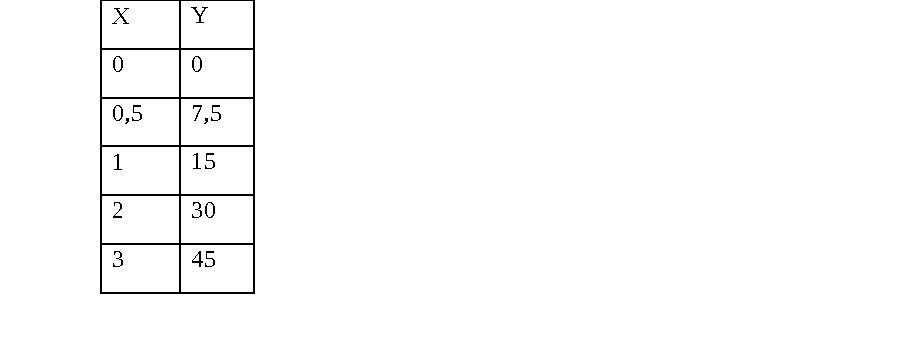
\includegraphics[width=0.45\textwidth]{capitulos/funcao_do_primeiro_grau/media/image3.pdf} 
    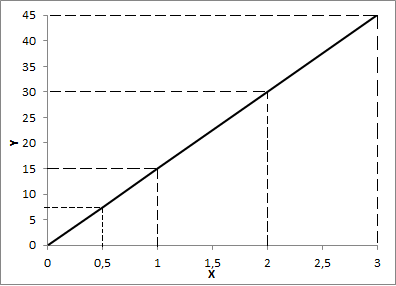
\includegraphics[width=0.45\textwidth]{capitulos/funcao_do_primeiro_grau/media/image4.png}
\end{figure}

Os valores de \textit{x} e \textit{y} formam pares ordenados (\textit{x,y}) que localizados no Plano Cartesiano, neste caso, formam uma \textbf{reta}. Como podemos usar qualquer \textit{x $ \in \mathbb{R} $, x $ \geq $  0} , a reta será contínua.

Nesse exemplo, na medida que a massa \textit{x} cresce, o custo \textit{y} também cresce, proporcionalmente. Ou seja, para cada incremento de \textit{1 kg}, o custo cresce \textit{15 reais} \qedsymbol{}
\end{texemplo}

\begin{texemplo}
Represente a função do Exemplo 2.2 em um gráfico cartesiano.

\textbf{Solução}: Dispondo alguns valores de \textit{x} e A em uma tabela, temos: 

\begin{figure}[H]
    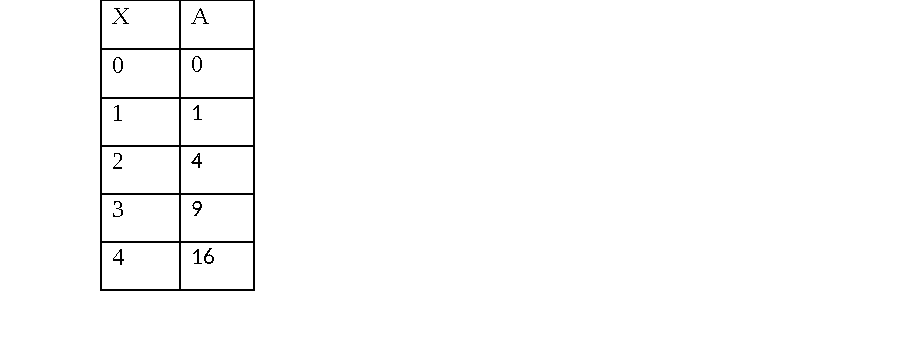
\includegraphics[width=0.45\textwidth]{capitulos/funcao_do_primeiro_grau/media/image5.pdf} 
    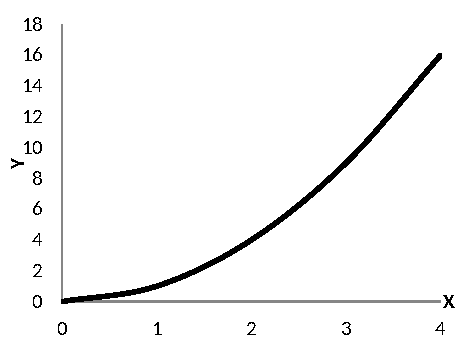
\includegraphics[width=0.45\textwidth]{capitulos/funcao_do_primeiro_grau/media/image6.pdf}
\end{figure}

Os valores de \textit{x} e \textit{A} formam pares ordenados (\textit{x,y}) que localizados no Plano Cartesiano, neste caso, formam uma \textbf{curva}. Como podemos usar qualquer \textit{x $ \in \mathbb{R} $  , x $ \geq $  0} , a curva será contínua.

Nesse exemplo, na medida que o lado \textit{x} cresce, a área \textit{A} também cresce, porém diferentemente do Exemplo 1, que tinha um crescimento constante. No primeiro incremento, a área cresceu \textit{1 cm\textsuperscript{2}}, no segundo \textit{3 cm\textsuperscript{2}}, no terceiro \textit{5 cm\textsuperscript{2}}. \qedsymbol{}
\end{texemplo}

\begin{texemplo}
Verifique se  -\textit{3x + y\textsuperscript{2} = 1} é uma função, de acordo com a Def. 2.1. Considere \textit{x $ \in \mathbb{R} $}.

\textbf{Solução}: A equação dada está na forma implícita (\textit{x} e \textit{y} estão no mesmo lado da igualdade). Para explicitar y, adicionamos (\textit{+3x}) em ambos os lados da equação, obtendo:

\textit{y\textsuperscript{2} = 1 + 3x.}

Aplicando raiz quadrada em ambos os lados da equação, temos:

 \( y= \pm \sqrt[]{1+3x} \)   .

Esta equação só terá valores reais para \textit{y}, se o radicando for um número nulo ou positivo. Então,

 \( 1+ 3x  \geq  0  \)      ou      \( x~  \geq  -1/3. \) 

\begin{figure}[H]
	\begin{Center}
		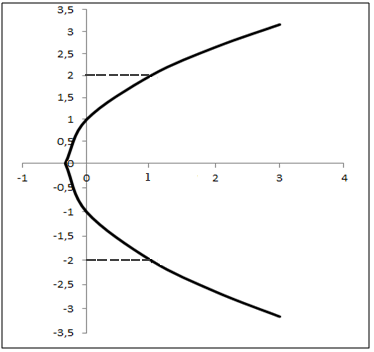
\includegraphics[width=3.9in,height=3.67in]{capitulos/funcao_do_primeiro_grau/media/image7.png}
	\end{Center}
\end{figure}

Observemos que para qualquer valor de \textit{x > -1/3}, teremos dois valores de \textit{y}. Por exemplo:

\tab Se \textit{x = 1}, teremos \textit{y = $ \pm $  2};  

\tab Se \textit{x = 2}, teremos   \( y= \pm \sqrt[]{7} \);

\tab Se \textit{x = 5}, teremos \textit{y = $ \pm $  4 }e assim por diante.   

Portanto, a equação dada não é uma função.  \qedsymbol{}
\end{texemplo}

\begin{caixa}
\textbf{Notação:}

Usa-se a notação \textit{y = f(x)} para referir-se à função \textit{f} de \textit{x}, onde \textit{x} é a variável independente e \textit{y = f(x)}  é a variável dependente de \textit{x}.

Por exemplo:   \textit{f(x) = x\textsuperscript{2}}        ou      \textit{f(x) = 3x - 2}.
\end{caixa}

\begin{caixa}
\begin{tdefinicao}
O \textit{domínio} de uma função \textit{y = f(x)} é o conjunto dos valores de \textit{x} nos quais a função é definida e denota-se:   \textit{D f(x).}
\end{tdefinicao}

\begin{tdefinicao}
A \textit{imagem} de uma função \textit{y = f(x)} é o conjunto dos valores de \textit{y }para os quais existem valores de \textit{x} correspondentes e denota-se : \textit{I\textsubscript{m} f(x).}
\end{tdefinicao}
\end{caixa}

\begin{texemplo}
Determine o domínio e a imagem da função \textit{ f(x) = x\textsuperscript{2} + 2.}

\textbf{Solução}:  Observemos que qualquer valor de \textit{x $ \in \mathbb{R} $} gera um valor de \textit{f(x)}. Então, 

\tab  \textit{Df(x)=$ \{ $ x $ \in \mathbb{R} $   } \textit{$ \} $ .}

Analisando a expressão da função, observamos que ela tem a soma de dois termos positivos (lembremos que para \textit{x\textsuperscript{2}}, teremos sempre \textit{x\textsuperscript{2}} > 0). Portanto, o menor valor possível de \textit{x\textsuperscript{2} + 2 } será \textit{2}, quando \textit{x = 0}. Então, 

\textit{I\textsubscript{m} f(x) = $ \{ $  y $ \epsilon $   \textbf{R}, y $ \geq $  2$ \} $ .}

\begin{figure}[H]
	\begin{Center}
		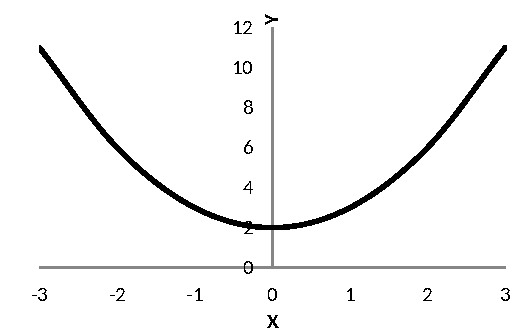
\includegraphics[width=3.5in,height=2.24in]{capitulos/funcao_do_primeiro_grau/media/image8.pdf}
	\end{Center}
\end{figure}

No gráfico de \textit{f(x)}, traçando \textit{retas verticais}, para qualquer \textit{x} teremos sempre um \textit{y} correspondente, o que indica que \textit{f(x)} é uma função.  

A imagem de \textit{f(x)} pode ser obtida traçando retas horizontais. Os valores de \textit{y}, pelos quais estas retas passarão, pertencem a imagem de \textit{f(x)}. Assim, a imagem desta função será o conjunto de números reais \textit{y }tal que  \textit{y $ \geq $  2 }\qedsymbol{}
\end{texemplo}

\begin{exercicios}
\exitem{} Localize os pontos no plano cartesiano:

\begin{multicols}{3}
a) \textit{A = (2,3)}

b) \textit{B = (-2,-3)}

c) \textit{C = (-3,3)}

d) \textit{D = (0,3)}

e)\textit{ E = (2,0)}

f) \textit{F = (0,-3)}
\end{multicols}

\exitem{} Qual é o valor de $x$ (abcissa) dos pontos sobre o eixo Y?

\exitem{} Qual é o valor de \textit{y} (ordenada) dos pontos sobre o eixo \textit{X} ?

\exitem{} Dada a função \textit{f(x) = 3x -1}, calcule:

\begin{multicols}{3}
a) \textit{f(0)}

b) \textit{f(-2)}

c) \textit{f(c+1)}

d) \textit{f(1)}

e) \textit{f(1/3)}

f) \textit{f(3-c)}
\end{multicols}

\exitem{} Dada a função \textit{f(x) = -2x +1/2}, calcule \textit{x} sendo:

\begin{multicols}{2}
a) \textit{f(x)=1/2} 

b) \textit{f(x)=1} 

c) \textit{f(x)=-3/4}

d) \textit{f(x)=4}
\end{multicols}

\exitem{} Faça o gráfico das funções com variáveis reais:

\begin{multicols}{3}
a) \textit{y = 3x}

b) \textit{f(x) = -3x +1 } 

c)  \textit{y = x\textsuperscript{2}}

d) \textit{y = x\textsuperscript{2} +1}

e)  \( g \left( x \right) =\frac{1}{x} \) 

f)  \( y=\frac{1}{x-1} \) 
\end{multicols}

\exitem{} Faça o gráfico dos dados das tabelas: 

\begin{multicols}{4}
\begin{table}[H]
a)

\begin{tabular}{p{0.2in}p{0.2in}}
\hline
%row no:1
\multicolumn{1}{|p{0.2in}}{X} & 
\multicolumn{1}{|p{0.2in}|}{Y} \\
\hhline{--}
%row no:2
\multicolumn{1}{|p{0.2in}}{-3} & 
\multicolumn{1}{|p{0.2in}|}{-6} \\
\hhline{--}
%row no:3
\multicolumn{1}{|p{0.2in}}{-2} & 
\multicolumn{1}{|p{0.2in}|}{-4} \\
\hhline{--}
%row no:4
\multicolumn{1}{|p{0.2in}}{-1} & 
\multicolumn{1}{|p{0.2in}|}{-2} \\
\hhline{--}
%row no:5
\multicolumn{1}{|p{0.2in}}{0} & 
\multicolumn{1}{|p{0.2in}|}{0} \\
\hhline{--}
%row no:6
\multicolumn{1}{|p{0.2in}}{1} & 
\multicolumn{1}{|p{0.2in}|}{2} \\
\hhline{--}
%row no:7
\multicolumn{1}{|p{0.2in}}{2} & 
\multicolumn{1}{|p{0.2in}|}{4} \\
\hhline{--}
%row no:8
\multicolumn{1}{|p{0.2in}}{3} & 
\multicolumn{1}{|p{0.2in}|}{6} \\
\hhline{--}
\end{tabular}
 \end{table}

\begin{table}[H]
b)

\begin{tabular}{p{0.2in}p{0.2in}}
\hline
%row no:1
\multicolumn{1}{|p{0.2in}}{X} & 
\multicolumn{1}{|p{0.2in}|}{Y} \\
\hhline{--}
%row no:2
\multicolumn{1}{|p{0.2in}}{-3} & 
\multicolumn{1}{|p{0.2in}|}{-5} \\
\hhline{--}
%row no:3
\multicolumn{1}{|p{0.2in}}{-2} & 
\multicolumn{1}{|p{0.2in}|}{-3} \\
\hhline{--}
%row no:4
\multicolumn{1}{|p{0.2in}}{-1} & 
\multicolumn{1}{|p{0.2in}|}{-1} \\
\hhline{--}
%row no:5
\multicolumn{1}{|p{0.2in}}{0} & 
\multicolumn{1}{|p{0.2in}|}{1} \\
\hhline{--}
%row no:6
\multicolumn{1}{|p{0.2in}}{1} & 
\multicolumn{1}{|p{0.2in}|}{3} \\
\hhline{--}
%row no:7
\multicolumn{1}{|p{0.2in}}{2} & 
\multicolumn{1}{|p{0.2in}|}{5} \\
\hhline{--}
%row no:8
\multicolumn{1}{|p{0.2in}}{3} & 
\multicolumn{1}{|p{0.2in}|}{7} \\
\hhline{--}
\end{tabular}
 \end{table}

\begin{table}[H]
c)

\begin{tabular}{p{0.2in}p{0.19in}}
\hline
%row no:1
\multicolumn{1}{|p{0.2in}}{X} & 
\multicolumn{1}{|p{0.19in}|}{Y} \\
\hhline{--}
%row no:2
\multicolumn{1}{|p{0.2in}}{-3} & 
\multicolumn{1}{|p{0.19in}|}{12} \\
\hhline{--}
%row no:3
\multicolumn{1}{|p{0.2in}}{-2} & 
\multicolumn{1}{|p{0.19in}|}{9} \\
\hhline{--}
%row no:4
\multicolumn{1}{|p{0.2in}}{-1} & 
\multicolumn{1}{|p{0.19in}|}{3} \\
\hhline{--}
%row no:5
\multicolumn{1}{|p{0.2in}}{0} & 
\multicolumn{1}{|p{0.19in}|}{1} \\
\hhline{--}
%row no:6
\multicolumn{1}{|p{0.2in}}{1} & 
\multicolumn{1}{|p{0.19in}|}{3} \\
\hhline{--}
%row no:7
\multicolumn{1}{|p{0.2in}}{2} & 
\multicolumn{1}{|p{0.19in}|}{9} \\
\hhline{--}
%row no:8
\multicolumn{1}{|p{0.2in}}{3} & 
\multicolumn{1}{|p{0.19in}|}{12} \\
\hhline{--}
\end{tabular}
 \end{table}

\begin{table}[H]
d)

\begin{tabular}{p{0.2in}p{0.19in}}
\hline
%row no:1
\multicolumn{1}{|p{0.2in}}{X} & 
\multicolumn{1}{|p{0.19in}|}{Y} \\
\hhline{--}
%row no:2
\multicolumn{1}{|p{0.2in}}{-3} & 
\multicolumn{1}{|p{0.19in}|}{5} \\
\hhline{--}
%row no:3
\multicolumn{1}{|p{0.2in}}{-2} & 
\multicolumn{1}{|p{0.19in}|}{2} \\
\hhline{--}
%row no:4
\multicolumn{1}{|p{0.2in}}{-1} & 
\multicolumn{1}{|p{0.19in}|}{1} \\
\hhline{--}
%row no:5
\multicolumn{1}{|p{0.2in}}{0} & 
\multicolumn{1}{|p{0.19in}|}{2} \\
\hhline{--}
%row no:6
\multicolumn{1}{|p{0.2in}}{1} & 
\multicolumn{1}{|p{0.19in}|}{5} \\
\hhline{--}
%row no:7
\multicolumn{1}{|p{0.2in}}{2} & 
\multicolumn{1}{|p{0.19in}|}{9} \\
\hhline{--}
%row no:8
\multicolumn{1}{|p{0.2in}}{3} & 
\multicolumn{1}{|p{0.19in}|}{14} \\
\hhline{--}
\end{tabular}
 \end{table}
\end{multicols}

\exitem{} Todas as funções do Ex.6 são funções, de acordo com a Def. 2.1?

\exitem{} A expressão  \( y = \pm \sqrt[]{x} \)    é uma função, de acordo com a Def. 2.1?

\exitem{} Faça o gráfico das funções usando uma tabela eletrônica ou um editor de gráficos computacional.

\begin{multicols}{3}
a) \textit{y = - 2x + 5}

b)  \( y=x^{2}-2x+1 \)

c) \textit{  \( y=x^{4}-x^{2}+4 \)}

d) \textit{y = x\textsuperscript{3} +1}

e) \( y=\frac{x+1}{x-1} \) \tab 

f) \( y^{2}+ x^{2}=4 \) 
\end{multicols}

\exitem{} Todas as expressões do Ex. 10 são funções, de acordo com a Def. 2.1?

\exitem{} Determine o domínio e a imagem das funções:

\begin{multicols}{3}
a) \textit{y = x}

b) \( f \left( x \right) =\frac{1}{x} \)

c) \( y=4-x^{2} \)

d)  \( f \left( x \right) =\sqrt[]{x} \)

e)  \( g \left( x \right) =-\sqrt[]{x} \)

f)  \( q \left( x \right) =\sqrt[]{x-4} \)
\end{multicols}

\item Faça os gráficos das funções do Ex. 12 usando uma ferramenta computacional.
\end{exercicios}

\section{Função do 1º grau}

Os exercícios da Seção 2 mostram que existem funções cujo gráfico é uma reta e outras apresentam curvas de diferentes formatos. Nessa seção, serão estudadas as funções cujos gráficos são retas.

Uma das características das retas é a \textit{taxa de variação (crescimento ou decrescimento) constante}. Isto significa que, para o mesmo incremento \textit{($ \Delta $ x) }em qualquer \textit{x}, o incremento \textit{($ \Delta $ y) }em \textit{y}, será o mesmo. 

\begin{texemplo}
Dada a reta \textit{f(x) = x +1 }   use o incremento \textit{$ \Delta $ x = 1 }  em

 (i) \textit{x\textsubscript{0} = 0;   }(ii)\textit{ x\textsubscript{1} = 2}  ; (iii) \textit{x\textsubscript{2} = 5 } e calcule os respectivos incrementos em \textit{y}. 

\textbf{Solução}: i) Usando o incremento em  \textit{x\textsubscript{0} = 0} :  

\textit{ x\textsubscript{0} + $ \Delta $ x = 0+1 = 1} .  

Calculando  \textit{f(x\textsubscript{0})=f(0)=0+1=1.}   Calculando a\textit{ f(x\textsubscript{0} + $ \Delta $ x)=f(1)=1+1=2.}

O incremento em \textit{y} será:\textit{  $ \Delta $ y =  f(x\textsubscript{0} + $ \Delta $ x)- f(x\textsubscript{0}) =  2 - 1 = 1.}

ii) Usando o incremento em  \textit{x\textsubscript{1} = 2} :  

\textit{x\textsubscript{1} + $ \Delta $ x = 2 +1  = 3} .  

Calculando  \textit{f(x\textsubscript{1})=f(2)=2+1=3.}   Calculando a\textit{ f(x\textsubscript{1} + $ \Delta $ x)=f(3)=3+1=4.}

O incremento em \textit{y} será:\textit{  $ \Delta $ y =  f(x\textsubscript{1} + $ \Delta $ x)- f(x\textsubscript{1}) =  4 - 3 = 1.  }

iii) Usando o incremento em  \textit{x\textsubscript{2} = 5 } 

\textit{x\textsubscript{2} + $ \Delta $ x = 5+1  = 6} .  

Calculando  \textit{f(x\textsubscript{2})=f(5)=5+1=6.}   Calculando a\textit{ f(x\textsubscript{2} + $ \Delta $ x)=f(6)=6+1=7.}

O incremento em \textit{y} será:\textit{  $ \Delta $ y =  f(x\textsubscript{2} + $ \Delta $ x)- f(x\textsubscript{2}) =  7 - 6 = 1.  }

Como podemos observar, o incremento \textit{$ \Delta $ y}  foi o mesmo, nos três casos analisados: \textit{$ \Delta $ y=1}

Faça um gráfico mostrando os incrementos \textit{$ \Delta $ x} e  nos valores de \textit{x} dados.\qedsymbol{}
\end{texemplo}

\begin{caixa}
\begin{tdefinicao}
Uma função polinomial do primeiro grau tem a forma

\textit{y = f(x) = ax + b} \tab (3.1)

onde \textit{a} e \textit{b} são números reais, \textit{x} e \textit{y} são variáveis reais.

O coeficiente \textit{a}  é chamado \textbf{coeficiente angular (inclinação)} e o \textit{b} \textbf{coeficiente linear}.
\end{tdefinicao}
\end{caixa}

\begin{texemplo}
Faça os gráficos das funções: (i)  \textit{ f(x) = x + 1  ;  }(ii) \textit{ g(x) = 2x + 1; }(iii) \textit{h(x) = 3x + 1.}

\textbf{Solução:} Elaborando tabelas para as três funções e localizando os pares ordenados no Plano Cartesiano, obtemos três retas.  

\begin{figure}[H]
	\begin{Center}
		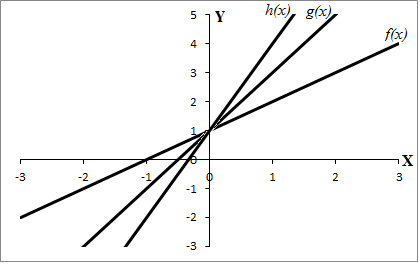
\includegraphics[width=4.38in,height=2.77in]{capitulos/funcao_do_primeiro_grau/media/image9.png}
	\end{Center}
\end{figure}

Observemos que as inclinações são diferentes, sendo que a diferença entre as três funções é o \textit{coeficiente angular}. Observemos que quanto maior o \textit{a} mais inclinada está a reta \qedsymbol{}
\end{texemplo}

\begin{caixa}
O coeficiente angular é a \textit{inclinação (ou taxa de crescimento)} da reta, dado pela expressão:

\begin{FlushRight}
 \( a=tg \left(  \theta  \right) =\frac{ \Delta y}{ \Delta x}=\frac{y_{i}-y_{i+1}}{x_{i}-x_{i+1}} \) \tab (3.2)
\end{FlushRight}

Onde \textit{i = 0,1,2,3,...} refere-se aos pontos de \textit{f(x)} e  é o ângulo que a reta faz com o eixo \textit{X}.
\end{caixa}

\begin{figure}[H]
	\begin{Center}
		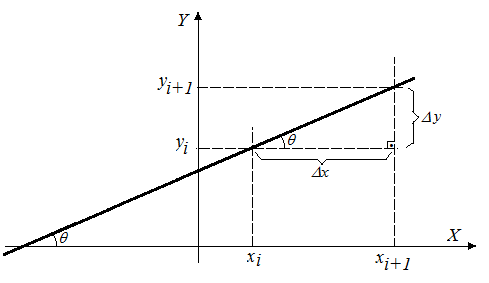
\includegraphics[width=5.09in,height=2.95in]{capitulos/funcao_do_primeiro_grau/media/image10.png}
	\end{Center}
\end{figure}

\begin{texemplo}
Faça os gráficos das funções: (i)  \textit{ f(x) = x + 1  ;  }(ii) \textit{ g(x) = x + 2; }(iii) \textit{h(x) = x + 3.}

\textbf{Solução:} Elaborando tabelas para as três funções e localizando os pares ordenados no Plano Cartesiano, obtemos três retas.

\begin{figure}[H]
	\begin{Center}
		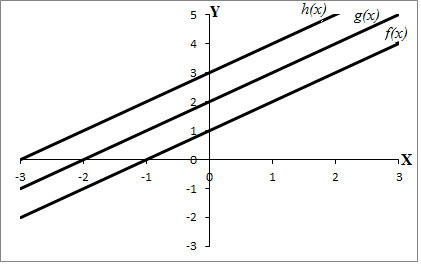
\includegraphics[width=4.39in,height=2.75in]{capitulos/funcao_do_primeiro_grau/media/image11.png}
	\end{Center}
\end{figure}

Observemos que todas têm a mesma inclinação, pois os coeficientes angulares são iguais: \textit{a = 1}.

Observemos também que quando calculamos as funções para \textit{x = 0} (pontos sobre o eixo \textit{Y}) o valor obtido é o coeficiente linear: \textit{f(0) = 1; g(0) = 2  }e\textit{  h(0) = 3}.  Podemos concluir que o \textit{coeficiente linear} é o valor do \textit{y}, nos pontos onde a reta corta o eixo \textit{Y}  \qedsymbol{}
\end{texemplo}

\begin{caixa}
O \textit{coeficiente linear} é o valor do \textit{y }(ordenada), no ponto (\textit{0,b}) onde a reta corta o eixo \textit{Y}  
\end{caixa}

\begin{texemplo}
Uma reta passa pelos pontos: \textit{P\textsubscript{1} = (1,2) }e\textit{ P\textsubscript{2} = (3,5):}

i) Calcule o coeficiente angular

ii) Calcule o coeficiente linear.

\textbf{Solução: }(i) Usando a Eq. (3.2) temos:

 \[ a=\frac{5-2}{3-1}=\frac{3}{2} \] 

(ii) Substituindo o valor de \textit{a} na Eq. (3.2), temos:

 \( y=\frac{3}{2}x+b \) \tab (3.3)

Como a reta passa pelos pontos \textit{P\textsubscript{1 }}e\textit{ P\textsubscript{2}}, as coordenadas desses pontos devem satisfazer a Eq. (3.3). Usando as coordenadas de\textit{ P\textsubscript{1} = (1,2) }na Eq. (3.3), temos:

\textit{\( 2=\frac{3}{2} \cdot 1+b \)}. Resolvendo para\textit{ b, }temos\textit{:}

\( b=\frac{1}{2} \)  

Observemos que se fosse utilizado o ponto \textit{P\textsubscript{2} = (3,5)} , obteríamos o mesmo valor de \textit{b}  \qedsymbol{}
\end{texemplo}

\subsection{Crescimento e decrescimento das funções do 1º grau}

O quadro abaixo define o que são funções crescentes e decrescentes:

\begin{caixa}
Seja \textit{y = f(x)} uma função definida no intervalo \textit{(x\textsubscript{0},x\textsubscript{n}).} 

Se \textit{f(x\textsubscript{i+1}) > f(x\textsubscript{i})} para qualquer \textit{x\textsubscript{i }} $ \in $  \textit{(x\textsubscript{0},x\textsubscript{n}} ) então \textit{f} é \textit{crescente} em \textit{(x\textsubscript{0},x\textsubscript{n}).}

Se \textit{f(x\textsubscript{i+1}) <  f(x\textsubscript{i})} para qualquer \textit{x\textsubscript{i }} $ \in $  \textit{(x\textsubscript{0},x\textsubscript{n})} então \textit{f}é  de\textit{crescente} em \textit{(a,b).}
\end{caixa}

 O quadro abaixo apresenta a relação entre coeficiente angular e crescimento da função do 1º grau:

\begin{caixa}
Se o \textit{coeficiente angular} é \textit{positivo} a reta é crescente.

Se o \textit{coeficiente angular} é \textit{negativo }a reta é decrescente.
\end{caixa}

\begin{texemplo}
Verifique se as retas são crescentes ou decrescentes. 

i) \textit{f(x) = 3x - 5}

ii) \textit{f(x) = - x + 2}

iii) \textit{4 = 3x -2y}

\textbf{Solução:}

(i) O coeficiente angular da reta é \textit{+3}. Portanto a reta é crescente para qualquer \textit{x $ \in \mathbb{R}$.}

(ii)  O coeficiente angular da reta é \textit{-1}. Portanto a reta é decrescente para qualquer \textit{x $ \in \mathbb{R} $.}

(iii) A equação está na forma implícita. Adicionando (\textit{+2y}) e (\textit{-4}) em ambos os lados, obtemos:

\textit{\tab 2y = 3x - 4. }Dividindo a equação por \textit{2}, obtemos:   \( y=\frac{3}{2}x-2 \) . 

O coeficiente angular da reta é \textit{+3/2}. Portanto a reta é crescente para qualquer \textit{x $\in \mathbb{R}.$}\qedsymbol{}
\end{texemplo}

\subsection{Domínio e imagem da função de 1º grau}

\begin{caixa}
As funções de 1º grau têm a expressão de um polinômio, cujas operações são possíveis para qualquer \textit{x} real. Assim, o domínio destas funções é:

\textit{Df(x)= $ \{ $ x $ \in \mathbb{R} $ $ \} $ } .

Como as funções de 1º grau são estritamente crescentes ou decrescentes e não tem descontinuidades, sua imagem é

\textit{Imf(x)= $ \{ $ y $ \in \mathbb{R} $  $ \} $ .}
\end{caixa}

\subsection{Raiz da função de 1º grau}

\begin{caixa}
\begin{tdefinicao}
	A raiz de uma função é o valor do \textit{x}, do ponto onde a função intercepta o eixo \textit{X}.
\end{tdefinicao}
\end{caixa}

A raiz das funções de 1º grau é determinada fazendo \textit{y=f(x)=0} na Eq. (3.1), de acordo com a Def. 3.2, pois os pontos sobre o eixo \textit{X}, tem \textit{y = 0}. Assim, 

\textit{0 = ax + b} . Resolvendo para \textit{x}, temos:

\begin{caixa}
 \( x=-\frac{b}{a} \) \tab (raiz da função de 1º grau)
\end{caixa}

\begin{texemplo}
Determine a raiz da função  \textit{5 = -2x - y}  e mostre-a no gráfico da função.

\textbf{Solução:} Mesmo com a equação na forma implícita, colocamos a exigência da Def. 3.1 \textit{y = 0}  na função dada e obtemos: 

\textit{\tab 5 = -2x - 0} .  Resolvendo para \textit{x}, temos   \textit{x = -5/2}, que é a raiz da função. 

\begin{figure}[H]
	\begin{Center}
		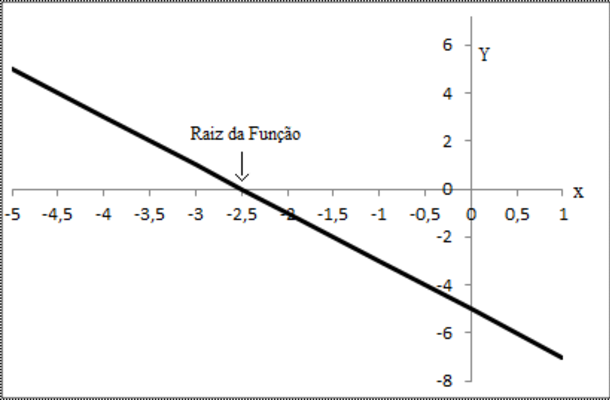
\includegraphics[width=4.41in,height=2.79in]{capitulos/funcao_do_primeiro_grau/media/image12.pdf}
	\end{Center}
\end{figure}

A Fig. 3.5 mostra a raiz da função no ponto (\textit{-5/2,0}) de interceptação do eixo \textit{X}  \qedsymbol{}
\end{texemplo}

\subsection{Sinal da função de 1º grau}

Lembremos que os valores de \textit{y} são os valores da função. Portanto, o sinal da função em algum ponto é o sinal das ordenadas, nos pontos da função.

\begin{texemplo}
Dada a função \textit{y = f(x) = x - 3}, determine o sinal da função para os seguintes valores de \textit{x: -1, 0, 1,2,3,4,5}.

\textbf{Solução}: Substituindo os valores de \textit{x} dados em \textit{f(x)}, obtemos os respectivos valores de \textit{y}, apresentados na tabela.

\begin{table}[H]
 			\centering
\begin{tabular}{p{0.69in}p{0.27in}p{0.27in}p{0.27in}p{0.27in}p{0.67in}p{0.29in}p{0.19in}}
\hline
%row no:1
\multicolumn{1}{|p{0.69in}}{X} & 
\multicolumn{1}{|p{0.27in}}{-1} & 
\multicolumn{1}{|p{0.27in}}{0} & 
\multicolumn{1}{|p{0.27in}}{1} & 
\multicolumn{1}{|p{0.27in}}{2} & 
\multicolumn{1}{|p{0.67in}}{3} & 
\multicolumn{1}{|p{0.29in}}{4} & 
\multicolumn{1}{|p{0.19in}|}{5} \\
\hhline{--------}
%row no:2
\multicolumn{1}{|p{0.69in}}{Y} & 
\multicolumn{1}{|p{0.27in}}{-4} & 
\multicolumn{1}{|p{0.27in}}{-3} & 
\multicolumn{1}{|p{0.27in}}{-2} & 
\multicolumn{1}{|p{0.27in}}{-1} & 
\multicolumn{1}{|p{0.67in}}{0} & 
\multicolumn{1}{|p{0.29in}}{+1} & 
\multicolumn{1}{|p{0.19in}|}{+2} \\
\hhline{--------}
%row no:3
\multicolumn{1}{|p{0.69in}}{Sinal de Y} & 
\multicolumn{1}{|p{0.27in}}{\textit{-}} & 
\multicolumn{1}{|p{0.27in}}{\textit{-}} & 
\multicolumn{1}{|p{0.27in}}{\textit{-}} & 
\multicolumn{1}{|p{0.27in}}{\textit{-}} & 
\multicolumn{1}{|p{0.67in}}{Sem sinal} & 
\multicolumn{1}{|p{0.29in}}{+} & 
\multicolumn{1}{|p{0.19in}|}{+} \\
\hhline{--------}

\end{tabular}
 \end{table}

Observemos que o sinal dos valores da função (\textit{y}) são negativos para \textit{x < 3} e positivos para \textit{x > 3}. A mudança do sinal ocorreu em \textit{x = 3}, que é a raiz da função.

\begin{figure}[H]
	\begin{Center}
		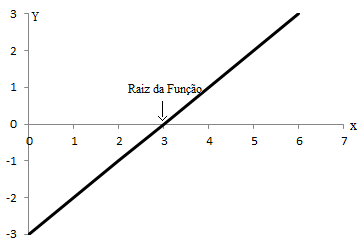
\includegraphics[width=3.75in,height=2.56in]{capitulos/funcao_do_primeiro_grau/media/image13.png}
	\end{Center}
\end{figure}

A visualização do sinal é evidente no gráfico, assim como a mudança do sinal a partir da raiz da função  \qedsymbol{}
\end{texemplo}

\begin{texemplo}
Determine o sinal das funções: (i)  \textit{ f(x) = x - 1} e  (ii)  \textit{ g(x) = -x - 1}.

\textbf{Solução}: No Exemplo 3.7 observamos que o sinal da função muda quando a função intercepta o eixo X (raiz da função). Então, vamos calcular as raízes das funções e ver a inclinação das mesmas.

\textbf{(i)} Raiz de \textit{f(x)}:    \( x=-\frac{b}{a}=-\frac{-1}{1}=1 \) . 

Como \textit{f(x)} é inclinada para a direita (crescente, pois \textit{a = 1 > 0}) , \textit{f(x) } é negativa se \textit{x < 1} e positiva se \textit{x > 1}.

\begin{figure}[H]
	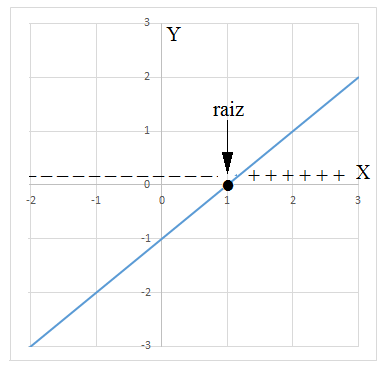
\includegraphics[width=0.45\textwidth]{capitulos/funcao_do_primeiro_grau/media/image14.png} 
	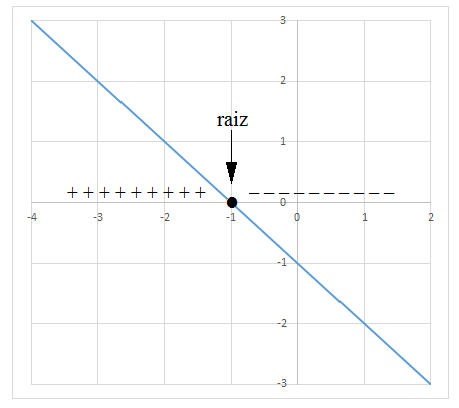
\includegraphics[width=0.45\textwidth]{capitulos/funcao_do_primeiro_grau/media/image15.png}
\end{figure}

\textbf{(ii)} Raiz de $g(x): x = -\frac{a}{b} = -\frac{-1}{-1} = -1$.

Como \textit{f(x)} é inclinada para a esquerda (decrescente, pois \textit{a = -1 < 0}) , \textit{f(x) } é positiva se \textit{x < -1} e negativa  se \textit{x > -1}  \qedsymbol{}
\end{texemplo}

\begin{caixa}
\textbf{SINAL DA FUNÇÃO DO 1º GRAU}

Seja \textit{y = f(x)=ax + b, }cuja raiz é\textit{  \( x_{r}=-\frac{b}{a} \)  .}

Se \textit{a > 0}  então:  \textit{f(x) }é \textbf{negativa } para\textit{ x < x\textsubscript{r}  }e  \textit{f(x) }é \textbf{positiva} para\textit{ x > x\textsubscript{r}.}

Se \textit{a < 0}  então:  \textit{f(x) }é \textbf{positiva } para\textit{ x < x\textsubscript{r}  }e  \textit{f(x) }é \textbf{negativa} para\textit{ x > x\textsubscript{r}.}
\end{caixa}

\subsection{Tipos especiais de retas}

\subsubsection{Função constante}

As \textit{retas horizontais} são chamadas funções constantes, pois não crescem nem decrescem. Seu coeficiente angular, pela Eq. (3.2) será nulo, portanto sua equação será:

\begin{caixa}
\textit{y = b, para b $ \in \mathbb{R} $}. \tab (3.4)
\end{caixa}

Observemos que para \textit{b = 0}, temos \textit{y = 0}, que é o próprio eixo \textit{X}.

Se \textit{f(x)=c}  o \textit{Df(x)=}$ \{ $ \textit{ x $\in \mathbb{R}$} $ \} $  e a imagem é    \textit{I\textsubscript{m}f(x) =} $ \{ $ \textit{ y $\in \mathbb{R}$} / \textit{y = b }$ \} $ .

\begin{texemplo}
Faça o gráfico das funções: 

i) \textit{y = 3} \tab (ii) \textit{y = -2}

\textbf{Solução:}

\begin{figure}[H]
	(i) 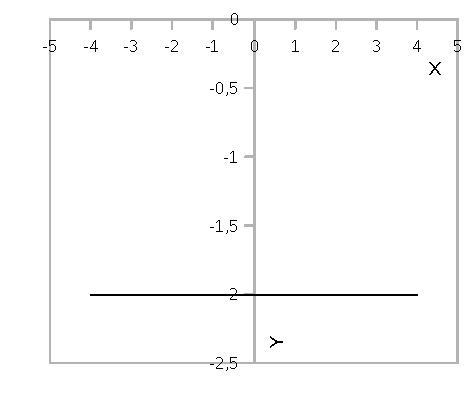
\includegraphics[width=0.45\textwidth]{capitulos/funcao_do_primeiro_grau/media/image16.pdf} 
	(ii) 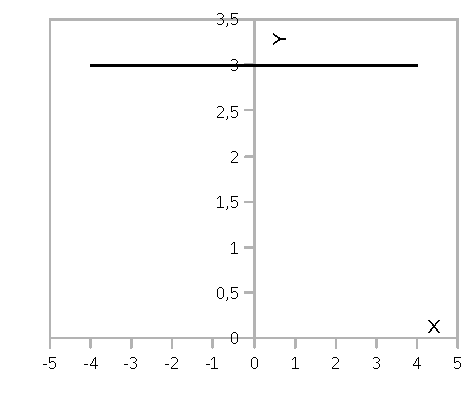
\includegraphics[width=0.45\textwidth]{capitulos/funcao_do_primeiro_grau/media/image17.pdf}
\end{figure}
\end{texemplo}

Todas as funções dadas são funções constantes (retas paralelas a \textit{X}, ou retas horizontais). Mesmo variando os valores de \textit{x}, os valores de \textit{y} permanecem constantes. \qedsymbol{} 

\subsubsection{Retas verticais}

Estas retas, de acordo com a definição de função (Def. 2.1) NÃO SÃO FUNÇÕES, pois para o mesmo \textit{x}, correspondem vários valores de \textit{y}. Tão pouco, são funções do 1º grau. Observemos que, não existe coeficiente angular, porque a Eq. (3.2) teria denominador nulo. Assim, a expressão para as retas verticais não deriva da forma da Eq.(3.1). 

A expressão para as retas verticais é construída com base no fato da abcissa ser constante para qualquer valor da ordenada, \textit{y}. Então:

\begin{caixa}
\textit{x = c}, onde  \textit{c} é uma constante. \tab (3.5)
\end{caixa}

\begin{texemplo}
Faça o gráfico das retas: 

i) \textit{x = 3} \qquad (ii) \textit{x = -1}

\textbf{Solução:}

\begin{figure}[H]
	i) 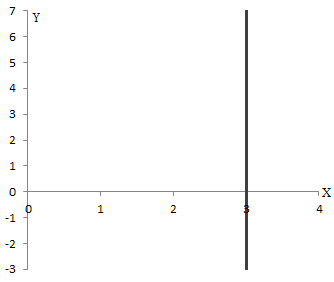
\includegraphics[width=0.45\textwidth]{capitulos/funcao_do_primeiro_grau/media/image18.png} 
	ii) 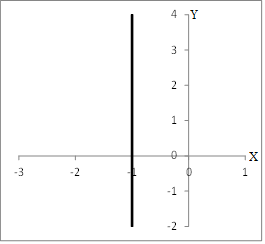
\includegraphics[width=0.45\textwidth]{capitulos/funcao_do_primeiro_grau/media/image19.png}
\end{figure}
\end{texemplo}

\subsubsection{Função identidade}

Esta função tem esse nome porque os valores de \textit{x} e \textit{y} são iguais. Sua expressão é:

\begin{caixa}
\textit{y = x}. \tab (3.6)
\end{caixa}

Se \textit{f(x) = x}  o domínio \textit{Df(x)=}$ \{ $ \textit{ x $ \in \mathbb{R} $} $ \} $  e a imagem é \textit{I\textsubscript{m}f(x) =} $ \{ $ \textit{ y $ \in \mathbb{R} $} $ \} $ \qedsymbol{}

\begin{texemplo}
Faça o gráfico da função  \textit{y = x}.

\textbf{Solução:} A função identidade divide na metade o 1º e o 3º quadrantes do Plano Cartesiano. O ângulo que esta reta faz com o eixo \textit{X} é \textit{45º }\qedsymbol{}

\begin{figure}[H]
	\begin{Center}
		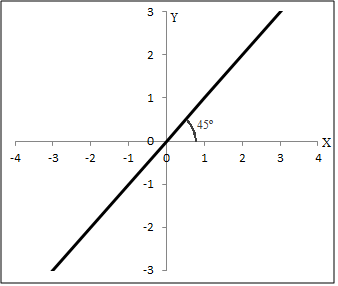
\includegraphics[width=3.52in,height=2.98in]{capitulos/funcao_do_primeiro_grau/media/image20.png}
	\end{Center}
\end{figure}
\end{texemplo}

\subsubsection{Função linear}

As funções do 1º grau, com \textit{a $ \neq $   0}  e \textit{b = 0} são chamadas funções lineares e têm a forma:

\begin{FlushRight}
\textit{y = ax.} \tab (3.7)
\end{FlushRight}

Se \textit{f(x) = ax}  o \textit{Df(x)=}$ \{ $ \textit{ x $ \in \mathbb{R} $} $ \} $  e a imagem é    \textit{I\textsubscript{m}f(x) =} $ \{ $ \textit{ y $\in \mathbb{R}$} $ \} $ .

\subsubsection{Função afim}

As funções do 1º grau, com \textit{a $ \neq $   0}  são chamadas \textbf{função afim} e têm a forma:

\begin{FlushRight}
\textit{y = ax + b.} \tab (3.8)
\end{FlushRight}

Se \textit{f(x) = ax} \textit{+ b} o \textit{Df(x)=}$ \{ $ \textit{ x $\in \mathbb{R}$} $ \} $  e a imagem é \textit{I\textsubscript{m}f(x) =} $ \{ $ \textit{ y $\in \mathbb{R}$} $ \} $ .

Observemos que as funções lineares são também funções afim.

\begin{texemplo}
Faça o gráfico da função  \textit{y = 4x}.

\textbf{Solução:} Como as funções lineares têm  \textit{b = 0}, então interceptam os eixos na origem (\textit{0,0}). O coeficiente angular igual a \textit{+4} indica que a função é crescente (inclinada para a direita), com inclinação \textit{+4}, portanto passará pelo ponto (\textit{1,4}). Colocando estes dados no Plano Cartesiano, obtemos o gráfico indicado na Fig. 3.14.

\begin{figure}[H]
	\begin{Center}
		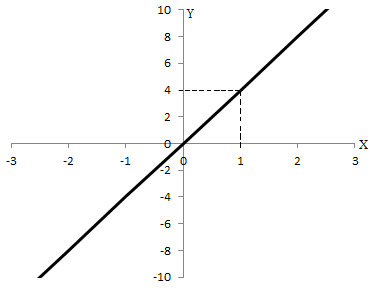
\includegraphics[width=3.12in,height=2.44in]{capitulos/funcao_do_primeiro_grau/media/image21.png} \qedsymbol{}
	\end{Center}
\end{figure}
\end{texemplo}

\subsection{Retas paralelas e perpendiculares}

\begin{caixa}
Sejam as retas    (\textit{r) :}   \textit{y = mx + b}   e   (\textit{s) :}   \textit{y = px + c}    . 

Se \textit{r} é \textbf{paralela} a \textit{s} então  \textit{m = p}. 

Se \textit{r} é \textbf{perpendicular} a  \textit{s}  então \( p=-\frac{1}{m} \)   .
\end{caixa}

\begin{exercicios}
\exitem{} Verifique se a dependência entre as grandezas mencionadas é de 1º grau:

\begin{enumerate}[label=\alph*)]
	\item Considere que a distribuição de adubo em uma lavoura é homogênea. A quantidade de adubo distribuída é proporcional a área de lavoura?

	\item A circunferência de um círculo é proporcional ao seu raio? E a área?

	\item O lixo produzido por uma cidade é proporcional ao número de habitantes?

	\item Uma caixa d’água é enchida por uma torneira, sempre com a mesma abertura. O volume de água da caixa é proporcional ao tempo? 

	\item No planejamento de uma festa, a quantidade de comida é proporcional à quantidade de pessoas?
\end{enumerate}

\exitem{} A tabela abaixo apresenta a deformação \textit{y } (\textit{cm}) de uma mola que está sendo distendida por massas \textit{m}, (\textit{g}) penduradas. Verifique se \textit{m} é proporcional a \textit{y}. 

\begin{table}[H]
 			\centering
\begin{tabular}{p{0.49in}p{0.29in}p{0.29in}p{0.29in}p{0.29in}p{0.29in}}
\hline
%row no:1
\multicolumn{1}{|p{0.49in}}{\textit{y}, (\textit{cm})} & 
\multicolumn{1}{|p{0.29in}}{0} & 
\multicolumn{1}{|p{0.29in}}{3} & 
\multicolumn{1}{|p{0.29in}}{6} & 
\multicolumn{1}{|p{0.29in}}{9} & 
\multicolumn{1}{|p{0.29in}|}{12} \\
\hhline{------}
%row no:2
\multicolumn{1}{|p{0.49in}}{\textit{m} (\textit{g})} & 
\multicolumn{1}{|p{0.29in}}{0} & 
\multicolumn{1}{|p{0.29in}}{50} & 
\multicolumn{1}{|p{0.29in}}{100} & 
\multicolumn{1}{|p{0.29in}}{150} & 
\multicolumn{1}{|p{0.29in}|}{200} \\
\hhline{------}

\end{tabular}
 \end{table}

\exitem{} Considerando que o custo de uma corrida de taxi \textit{(y)} depende de um valor fixo \textit{(b)}, referente à hora do dia, do preço por quilômetro percorrido (\textit{p}) e da quilometragem percorrida (\textit{x}). Fazendo \textit{b = 5,00} reais e \textit{p = 1,5} reais, determine uma função para o custo \textit{y(x)} de uma corrida.

\exitem{} Determine uma função que relacione o custo dos azulejos para revestir uma parede com \textit{x} \textit{m\textsuperscript{2}}, sendo que o preço de \textit{1} \textit{m\textsuperscript{2}}   de azulejo é \textit{p}.

\exitem{} O custo (\textit{C}) da carne usada para um churrasco depende do preço da carne (\textit{p}), da quantidade de carne comprada (\textit{x}) e da gasolina gasta para ir ao supermercado (\textit{b}). Faça uma função \textit{C(x)}.

\exitem{} O custo (\textit{C}) para produzir uma certa mercadoria é a soma dos custos fixos (\textit{CF}) e dos variáveis (\textit{a}) , aqueles que dependem da quantidade produzida (\textit{x}). Faça uma função \textit{C(x)}.

\exitem{} Determine os coeficientes angular e linear das retas que passam pelos pontos dados e construa a função do 1º grau:

\begin{multicols}{2}
	a) \textit{P\textsubscript{1} = (-1,0)}  e  \textit{P\textsubscript{2} = (3,2)}

	b) \textit{P\textsubscript{1} = (0,3)}  e  \textit{P\textsubscript{2} = (-3,0)}

	c) \textit{P\textsubscript{1} = (2,-2)}  e  \textit{P\textsubscript{2} = (-2,2)}

	d) \textit{P\textsubscript{1} = (3,3)}  e  \textit{P\textsubscript{2} = (5,3)}
\end{multicols}

\exitem{} Para produzir 5 peças de uma certa mercadoria foram gastos R$\$$  15,00. Para produzir 12 peças foram gastos R$\$$  35,00.  Supondo que os custos são proporcionais ao número de peças:

a) Determine uma função de 1º grau que relacione custos e número de peças

b) Determine o custo para 30 peças. 

\exitem{} Determine o coeficiente angular das funções e verifique se são crescentes ou decrescentes:

\begin{multicols}{2}
a) \textit{3x + y = 3}

b)  \( \frac{1}{2}x+y=4 \)

c)  \( \frac{3}{2}y+x=\frac{2}{3} \)

d)  \( \frac{x-y}{2}=3 \)
\end{multicols}

\exitem{} Dados os pontos da tabela, verifique se eles estão alinhados. Se estiverem, determine a equação da função linear e faça o gráfico.

\begin{multicols}{2}
\begin{table}[H]
\begin{tabular}{p{0.2in}p{0.18in}p{0.19in}p{0.16in}p{0.1in}}
\hline
%row no:1
\multicolumn{1}{|p{0.2in}}{X} & 
\multicolumn{1}{|p{0.18in}}{0} & 
\multicolumn{1}{|p{0.19in}}{1} & 
\multicolumn{1}{|p{0.16in}}{3} & 
\multicolumn{1}{|p{0.1in}|}{6} \\
\hhline{-----}
%row no:2
\multicolumn{1}{|p{0.2in}}{Y} & 
\multicolumn{1}{|p{0.18in}}{1} & 
\multicolumn{1}{|p{0.19in}}{3/2} & 
\multicolumn{1}{|p{0.16in}}{5/2} & 
\multicolumn{1}{|p{0.1in}|}{4} \\
\hhline{-----}
\end{tabular}
 \end{table}

\begin{table}[H]
\begin{tabular}{p{0.2in}p{0.18in}p{0.19in}p{0.16in}p{0.16in}}
\hline
%row no:1
\multicolumn{1}{|p{0.2in}}{X} & 
\multicolumn{1}{|p{0.18in}}{0} & 
\multicolumn{1}{|p{0.19in}}{1} & 
\multicolumn{1}{|p{0.16in}}{2} & 
\multicolumn{1}{|p{0.16in}|}{3} \\
\hhline{-----}
%row no:2
\multicolumn{1}{|p{0.2in}}{Y} & 
\multicolumn{1}{|p{0.18in}}{1,5} & 
\multicolumn{1}{|p{0.19in}}{2,5} & 
\multicolumn{1}{|p{0.16in}}{3,5} & 
\multicolumn{1}{|p{0.16in}|}{4,6} \\
\hhline{-----}
\end{tabular}
 \end{table}
\end{multicols}

\exitem{} Considere um quadrado cujos vértices estão nos pontos \textit{V\textsubscript{1} = (0,0)} ;   \textit{V\textsubscript{2} = (0,4);  V\textsubscript{3} = (4,4)}  e  \textit{V\textsubscript{4} = (4,0). }Determine equações para as retas correspondentes a cada lado do quadrado.

\exitem{} Considere um triângulo cujos vértices estão nos pontos \textit{V\textsubscript{1}=(1,1)} ; \textit{V\textsubscript{2}=(4,1) }e\textit{ V\textsubscript{3}=(1,4). }Determine equações para as retas correspondentes a cada lado do triângulo.

\exitem{} Dadas as equações de retas, faça o gráfico usando somente as informações fornecidas pelos coeficientes angular e linear (não use tabela):

\begin{multicols}{2}
a) \textit{y = -x + 1}

b) \textit{y = 4x}

c) \textit{y = -x}

d)  \textit{y = 2x - 3}

e) \textit{y = 1}

f) \textit{x = 1}
\end{multicols}

\exitem{} Construa a equação e faça um esboço do gráfico das retas \textit{y = ax + b}, com as informações dadas:

\begin{multicols}{2}
a) \textit{a = 2} e \textit{b = 1}

b) \textit{a = -1}  e passa em \textit{(1,0)}

c) passa em \textit{(0,0)} e tem inclinação \textit{-2}

d) é constante e passa em \textit{(2,3)}

e)  $\theta = 45\degree$ e \textit{b = -1}

f)  $\theta = 120\degree$ e passa em \textit{(0,3)}
\end{multicols}

\exitem{} a) Um motoqueiro cobra R$\$$  3,00 por viagem, para entregar até cinco pizzas. Sabendo que o custo de uma pizza é R$\$$  40,00, faça uma função que dê o custo de 1 a 5 pizzas. Faça o gráfico da função.

b) Refaça a função para o custo de uma pizza é R$\$$  50,00. Faça o gráfico e compare com a reta da letra (a).

\exitem{} Analise os coeficientes angular e linear das retas. Determine se as retas crescem ou decrescem e o ponto de intersecção com o eixo Y. Faça um esboço do gráfico com base nessa análise.

\begin{multicols}{3}
a) \textit{y = 3x + 5}

b) \textit{y = -2,3x - 1}

c)\textit{y = 2x - 1, 3}

d) \textit{y = -5,2x + 2,3}

e) \textit{y = -1, 3x + 2}

f) \textit{y = -4, 1x-5}
\end{multicols}

\exitem{} Nas retas que passam pelos pontos $P_1$ e $P_2$, determine se a reta cresce ou decresce e o ponto em que a reta intercepta o eixo Y:

\begin{multicols}{2}
a) \textit{P\textsubscript{1 }=(1,1) }e \textit{P\textsubscript{2 }=(2,4)}

b)\textit{ P\textsubscript{1}=(1,6) }e \textit{P\textsubscript{2 }=(5,3)}

c)\textit{ P\textsubscript{1}=(2,8) }e \textit{P\textsubscript{2 }=(7,1)}

d)\textit{ P\textsubscript{1}=(6,1) }e \textit{P\textsubscript{2 }=(1,3)}
\end{multicols}

\exitem{}  A fabricação de um produto implica em custos de materiais, energia, mão de obra, encargos sociais e impostos comerciais. Para uma determinada quantidade do produto, vamos considerar os custos de mão de obra como custo fixo, no valor de R$\$$  20,00. Considerando que os custos de materiais, energia e impostos são de R$\$$  150,00, para produzir uma unidade do produto:

a) Construa uma tabela relacionando o número de unidades do produto e o custo total.

b) Faça um gráfico com os dados da tabela.

c) Determine uma equação para relacionar o número de unidades do produto e o custo total.

d) Determine o coeficiente angular e o linear. Qual é o significado destes coeficientes no problema?

\exitem{} Uma agência de pesquisa estatística encontrou os percentuais de voto (V) mostrados na tabela abaixo para os candidatos A e B.

\begin{table}[H]
 			\centering
\begin{tabular}{p{0.26in}p{0.73in}p{0.83in}p{0.83in}}
%row no:1
\multicolumn{1}{p{0.26in}}{Data} & 
\multicolumn{1}{p{0.73in}}{Tempo(dias)} & 
\multicolumn{2}{p{0.83in}}{V ($\%$ )} \\
\hhline{~~~~}
%row no:2
\multicolumn{1}{p{0.26in}}{} & 
\multicolumn{1}{p{0.73in}}{} & 
\multicolumn{1}{p{0.83in}}{Candidato (A)} & 
\multicolumn{1}{p{0.83in}}{Candidato (B)} \\
\hhline{~~~~}
%row no:3
\multicolumn{1}{p{0.26in}}{01/07} & 
\multicolumn{1}{p{0.73in}}{1} & 
\multicolumn{1}{p{0.83in}}{35} & 
\multicolumn{1}{p{0.83in}}{30} \\
\hhline{~~~~}
%row no:4
\multicolumn{1}{p{0.26in}}{01/08} & 
\multicolumn{1}{p{0.73in}}{32} & 
\multicolumn{1}{p{0.83in}}{37} & 
\multicolumn{1}{p{0.83in}}{32} \\
\hhline{~~~~}
%row no:5
\multicolumn{1}{p{0.26in}}{01/09} & 
\multicolumn{1}{p{0.73in}}{63} & 
\multicolumn{1}{p{0.83in}}{46} & 
\multicolumn{1}{p{0.83in}}{40} \\
\hhline{~~~~}

\end{tabular}
 \end{table}

a) Faça um gráfico do percentual de voto (V) pelo tempo (t) para os dois candidatos, considerando o período 1/07 a 1/09.

b) Considere o percentual de voto uma função linear em cada mês e determine a função da reta do mês de julho. Com esta função, calcule o percentual para o dia 20 de julho.

c) Se a variável V mantiver em setembro a mesma tendência de agosto, para os dois candidatos, quais serão os percentuais de voto no dia 16 de setembro?
\end{exercicios}

\section{Aplicações de funções do 1º grau }

\subsection{Produção de bens: custo fixo + custo variável}

A produção de bens, seja na indústria ou na agricultura, apresenta custos variáveis e fixos. Os primeiros dependem da quantidade de bens produzidos e os últimos não dependem. Por exemplo, na produção de vinho, o custo das garrafas, matéria prima (uva), impostos, energia, água e produtos de limpeza são \textbf{variáveis}, ou seja, dependem da quantidade produzida. Quanto mais litros de vinhos forem produzidos, estes custos aumentarão proporcionalmente. Enquanto que o custo do aluguel, mão-de-obra, o equipamento (pipas, bomba, baldes, máquina de colocar rolhas,...) são \textbf{constantes} até uma certa quantidade de litros produzidos. 

Um modelo linear pode ser usado para modelar a produção de bens:

\begin{FlushRight}
\textit{\tab C(x) = p} \textit{x + CF} \tab (4.1)
\end{FlushRight}

Onde \textit{C(x) }é o custo total\textit{ (R$\$$ ), x }é a quantidade produzida (\textit{unidades})\textit{, p }é o custo variável por unidade produzida\textit{ (R$\$$ /unidade) }e\textit{ CF }é o custo fixo\textit{ (R$\$$ ).}

Observemos que a Eq. 4.1 é uma função afim, onde \textit{p} e \textit{CF} são os coeficientes angular e linear, respectivamente.

A Receita (ou ganhos com a venda do bem produzido) é proporcional à quantidade produzida e vendida. Assim, a função receita é uma função linear:

\begin{FlushRight}
\textit{R(x) = PV } \textit{x} \tab (4.2)
\end{FlushRight}

Onde \textit{R(x)} é a receita (\textit{R$\$$ }) e \textit{PV} é o preço de venda de cada bem (\textit{R$\$$ /unidade}).

Para determinar o Lucro da atividade, fazemos a diferença entre a receita e o custo de produção. 

\begin{Center}
\textit{L(x)= R(x) - C(x) = PVx -(p }\textit{x + CF)} ou
\end{Center}

\textit{L(x)=  (PV  - p)x - CF}. \tab (4.3)

Observemos que a Eq. 4.3 também é uma função afim.

Considere que para produzir um litro de vinho o custo variável por unidade é \textit{p = R$\$$  4,50}, o custo fixo é \textit{CF = R$\$$  2.000,00} e o preço de venda é \textit{PV = R$\$$  10,00}.

\begin{enumerate}
	\item Substitua os valores de \textit{p}, \textit{CF} e \textit{PV} nas Eqs. 4.1, 4.2 e 4.3  e faça os gráficos das funções \textit{C}, \textit{R} e \textit{L}, no mesmo plano cartesiano.

	\item Calcule quantos litros de vinho deverão ser produzidos para que a receita seja equivalente aos custos \qedsymbol{}
\end{enumerate}

\subsection{Produção de Lixo}

A Tabela abaixo apresenta dados sobre a produção de lixo doméstico em Chapecó em 2004, 2007 e 2012.

\begin{table}[H]
 			\centering
\begin{tabular}{p{1.67in}p{0.88in}p{1.28in}p{1.28in}}
\hline
%row no:1
\multicolumn{1}{|p{1.67in}}{Tempo, \textit{t} (anos)} & 
\multicolumn{1}{|p{0.88in}}{2004} & 
\multicolumn{1}{|p{1.28in}}{2007} & 
\multicolumn{1}{|p{1.28in}|}{2012} \\
\hhline{----}
%row no:2
\multicolumn{1}{|p{1.67in}}{População, \textit{h} (habitantes)} & 
\multicolumn{1}{|p{0.88in}}{165.220} & 
\multicolumn{1}{|p{1.28in}}{168.113} & 
\multicolumn{1}{|p{1.28in}|}{180.000} \\
\hhline{----}
%row no:3
\multicolumn{1}{|p{1.67in}}{Resíduos domésticos, \textit{R}    { (kg/hab./dia)}} & 
\multicolumn{1}{|p{0.88in}}{0,405} & 
\multicolumn{1}{|p{1.28in}}{0,630} & 
\multicolumn{1}{|p{1.28in}|}{0,855} \\
\hhline{----}

\end{tabular}
 \end{table}

Fonte: Abrelpe; MMA\tab (Dados citados pelas alunas Ana C. Maccari e Cristiane L. da Silva  no trabalho de Cálculo Numérico, Curso de Engenharia Ambiental, 2º/2014)

\begin{enumerate}
	\item Verifique se a população cresce linearmente com o tempo.

	\item Verifique se a produção de resíduos domésticos/habitante/dia cresce linearmente com o tempo.

	\item Considerando que \textit{R(h)} é linear entre 2007 e 2016, faça a previsão da \textit{R(2016)} \qedsymbol{}
\end{enumerate}

\subsection{Modelo Mola-massa}

Um sistema mola-massa é ilustrado na figura abaixo uma mola é distendida por massas \textit{m}, (\textit{g}) que causam deformações  \textit{y } (\textit{cm}). A posição \textit{y\textsubscript{o}} \textit{= 0} corresponde ao estado da mola sem massa. A cada massa \textit{m\textsubscript{i}} colocada corresponde uma posição \textit{y\textsubscript{i}} (deformação da mola), sendo \textit{i = 0,1,2,3,.. n} , o número de massas. Para o regime elástico (valores de \textit{m}, para os quais a mola ainda volta na posição \textit{y\textsubscript{o}}) as posições \textit{y} são proporcionais às massas \textit{m}. Considerando o conceito de força peso, que é a força com que a terra atrai as massas, temos

\textbf{F}\textit{ = m$ \cdot $  }\textbf{g}

Onde \textit{m} é a massa (\textit{g})  \textbf{g} a aceleração da gravidade (\textit{m/s\textsuperscript{2}}).

A relação entre \textit{F} e \textit{y}  é uma função de 1º grau, conhecida como Lei de Hooke

\textit{\tab F(y) = k y} ,   

onde \textit{k} é uma constante característica da mola. Observemos que \textit{k} é o coeficiente angular da função e neste caso, tem um significado físico: a $``$dureza$"$  da mola.

\begin{figure}[H]
	\begin{Center}
		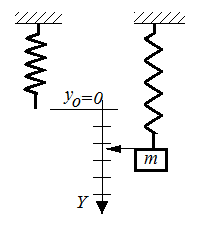
\includegraphics[width=2.06in,height=2.38in]{capitulos/funcao_do_primeiro_grau/media/image22.png}
	\end{Center}
\end{figure}

\begin{enumerate}
	\item Considere molas com \textit{k = 1,2 e 3}. Calcule as deformações \textit{y} para as massas 

\textit{m = 0,50,100,150 }e\textit{ 200 g}. (considere \textbf{g}\textit{ = 10} \textit{m/s\textsuperscript{2}})

	\item Faça um gráfico e compare as retas.

	\item Qual é a mola mais $``$dura$"$  \qedsymbol{}
\end{enumerate}

\subsection{Locação de carros}

A consulta a um site de locação de carros resultou nos dados da tabela abaixo. 

\begin{table}[H]
 			\centering
\begin{tabular}{p{0.88in}p{1.28in}}
\hline
%row no:1
\multicolumn{1}{|p{0.88in}}{Nº de diárias} & 
\multicolumn{1}{|p{1.28in}|}{Valor cobrado (R$\$$ )} \\
\hhline{--}
%row no:2
\multicolumn{1}{|p{0.88in}}{\Centering 1} & 
\multicolumn{1}{|p{1.28in}|}{\Centering 83} \\
\hhline{--}
%row no:3
\multicolumn{1}{|p{0.88in}}{\Centering 2} & 
\multicolumn{1}{|p{1.28in}|}{\Centering 166} \\
\hhline{--}
%row no:4
\multicolumn{1}{|p{0.88in}}{\Centering 3} & 
\multicolumn{1}{|p{1.28in}|}{\Centering 249} \\
\hhline{--}
%row no:5
\multicolumn{1}{|p{0.88in}}{\Centering 4} & 
\multicolumn{1}{|p{1.28in}|}{\Centering 332} \\
\hhline{--}
%row no:6
\multicolumn{1}{|p{0.88in}}{\Centering 5} & 
\multicolumn{1}{|p{1.28in}|}{\Centering 415} \\
\hhline{--}

\end{tabular}
 \end{table}

\begin{enumerate}
	\item Verifique se o valor cobrado (\textit{V}) é proporcional ao número de diárias (\textit{d}). Faça um modelo matemático que relacione \textit{V} e \textit{d}. Calcule \textit{V} para um aluguel de sete dias.

	\item Como ficaria este modelo se a locadora cobrasse uma taxa de lavagem de R$\$$  25,00.

	\item Outro sistema de aluguel considera uma taxa fixa de R$\$$  40,00, mais R$\$$  1,30 por quilômetro rodado. Faça um modelo matemático para este sistema de locação.

	\item Considerando a locação por quilômetro rodado (letra (d)), se um locador pretende ficar 3 dias com o carro, quanto quilômetros ele teria que rodar para que o custo seja equivalente ao do modelo da letra (c) ?

	\item Verifique qual é o sistema de locação mais vantajoso para uma semana de locação, com 400 km rodados.
\end{enumerate}

\subsection{Orçamento de Churrasco}

Consideremos as seguintes hipóteses de consumo para um churrasco:

- 450 g de carne por pessoa, 

- preço médio da carne: PM,

- custo da salada: 20$\%$  do custo da carne.

O custo médio de carne e salada por pessoa (\textit{p}) pode ser calculado fazendo:

\textit{p} = custo da carne + custo salada      

\textit{p = 0,450 $ \cdot $  PM  + 0,450 $ \cdot $  PM $ \cdot $  0,2 = 1,2 $ \cdot $  0,450 $ \cdot $  PM}   ou

\textit{p =  0,54 PM}

O custo de um churrasco (\textit{C}) para um grupo de pessoas depende do número de pessoas (\textit{x}), do custo da carne e salada por pessoa (\textit{p}) e da taxa de limpeza (\textit{b}) do local do churrasco.

\begin{FlushRight}
\textit{C(x) = p} \textit{x + b}. \tab (4.4)
\end{FlushRight}

\begin{enumerate}
	\item Qual é o custo de um churrasco para \textit{10} pessoas, considerando o preço médio da carne \textit{PM = R$\$$  18,00}.

	\item Que modificação na Eq. 4.4 deve ser implementada para incluir o custo da  gasolina (\textit{g}) usada para buscar os mantimentos?

	\item Que modificação na Eq. 4.4 deve ser implementada para incluir o custo da  sobremesa (\textit{SM})?
\end{enumerate}

\subsection{Deslocamento com velocidade constante}

As funções de 1º grau são úteis para modelar vários problemas de Física, como por exemplo o deslocamento de um carro em uma estrada retilínea, com velocidade constante. A velocidade (\textit{v}) é definida como a razão entre a variação da distância percorrida (\textit{x}) pela variação de tempo (\textit{t}):

\begin{FlushRight}
 \( v=\frac{ \Delta x}{ \Delta t} \) \tab (4.5)
\end{FlushRight}

Se  \textit{x\textsubscript{f}  }e\textit{ x\textsubscript{i}} são as posições final e inicial do carro (ver Fig. 4.6.1), substituindo \textit{$ \Delta $ x=x\textsubscript{f} - x\textsubscript{i}} , na Eq. (4.5), temos

\begin{FlushRight}
\textit{x\textsubscript{f} = v$ \cdot $ $ \Delta $ x + x\textsubscript{i}} \tab (4.6)
\end{FlushRight}

\begin{figure}[H]
	\begin{Center}
		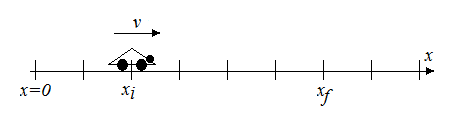
\includegraphics[width=4.8in,height=1.33in]{capitulos/funcao_do_primeiro_grau/media/image23.png}
	\end{Center}
\end{figure}

Se o tempo inicial for zero  \textit{$ \Delta $ x = t , }onde t é o tempo de deslocamento e \textit{x\textsubscript{f}}   é a posição final, ou seja, uma função de \textit{x(t)}. Então,

\begin{FlushRight}
\textit{X(t) = v$ \cdot $ t + x\textsubscript{i}} \tab (4.7)
\end{FlushRight}

\begin{enumerate}
	\item Determine a posição de um carro que partiu do quilômetro \textit{10} com velocidade constante \textit{80 km/h} e andou durante \textit{3 h}.

	\item Quanto tempo esse carro precisará rodar nessa velocidade para chegar no quilômetro 270 ?
\end{enumerate}

\subsection{Temperatura no interior de uma parede}

Consideremos que a parede de uma casa está sujeita a temperaturas diferentes e constantes, na superfície interna e externa da casa, durante um período de tempo. Se as temperaturas forem mantidas, a distribuição de temperatura no interior da parede será linear. 

\begin{figure}[H]
	\begin{Center}
		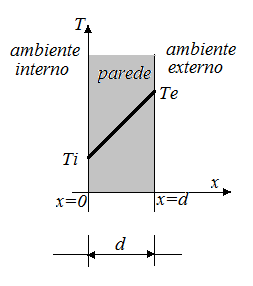
\includegraphics[width=2.64in,height=2.98in]{capitulos/funcao_do_primeiro_grau/media/image24.png}
	\end{Center}
\end{figure}

Seja \textit{d} a espessura da parede. Com base no sistema de coordenadas mostrado na figura acima, dois pontos da reta \textit{T(x)} são conhecidos. Então, podemos calcular o coeficiente angular: 

\begin{FlushRight}
 \( a=\frac{T_{e}-T_{i}}{ \Delta x}=\frac{ \Delta T}{d} \) \tab (4.8)
\end{FlushRight}

Como a reta intercepta o eixo das ordenadas em \textit{T = T\textsubscript{i}}  temos:

\begin{FlushRight}
 \( T \left( x \right) =\frac{ \Delta T}{d}x+T_{i} \) \tab (4.9)
\end{FlushRight}

\begin{enumerate}
	\item Determine uma função  \textit{T(x) }em uma parede, sabendo que \textit{45ºC } e \textit{25ºC} são as temperaturas externa interna da casa, respectivamente e a espessura da parede é de \textit{15 cm}.

	\item Usando a função do item (a), calcule a temperatura em \textit{5} \textit{cm}, \textit{7,5} \textit{cm} e \textit{10 cm}.
\end{enumerate}

\section{RESPOSTAS DOS EXERCÍCIOS PROPOSTOS}

\begin{respostas}{2}
\begin{figure}[H]
\ansitem{}

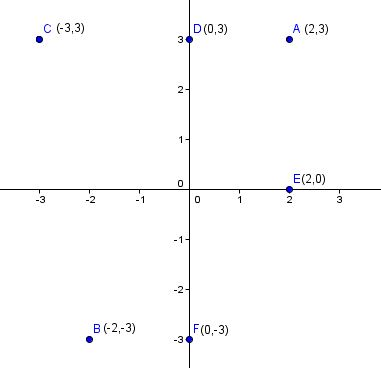
\includegraphics[width=3.2in,height=2.52in]{capitulos/funcao_do_primeiro_grau/media/image25.jpeg}
\end{figure}
\ansitem{}  \( x=0 \) 

\ansitem{}  \( y=0 \) 

\ansitem{}

\begin{multicols}{3}
a)  \( f \left( 0 \right) =-1 \)

b)  \( f \left( -2 \right) =-7 \)

c)  \( f \left( c+1 \right) =3c+2 \)

d)  \( f \left( 1 \right) =2 \)

e)  \( f \left( 1/3 \right) =0 \) 

f)  \( f \left( 3-c \right) =-3c+8 \) 
\end{multicols}

\ansitem{}

\begin{multicols}{2}
a)  \( x= 0  \)

b) \( x=-1/4 \)

c)  \( x=5/8 \)

d)  \( x=-7/4 \)
\end{multicols}

\begin{figure}[H]
	\ansitem{}

	a) 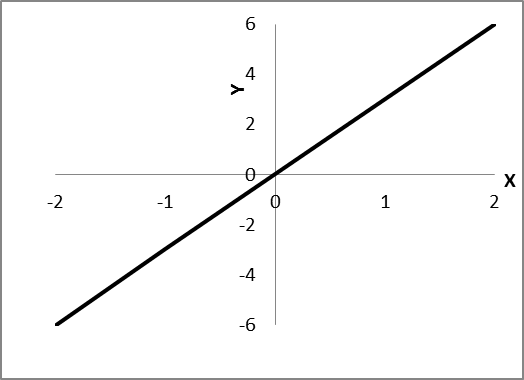
\includegraphics[width=0.45\textwidth]{capitulos/funcao_do_primeiro_grau/media/image26.png} 
	b) 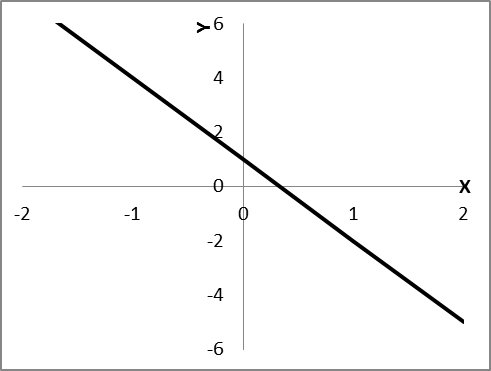
\includegraphics[width=0.45\textwidth]{capitulos/funcao_do_primeiro_grau/media/image27.png}
\end{figure}

\begin{figure}[H]
	c) 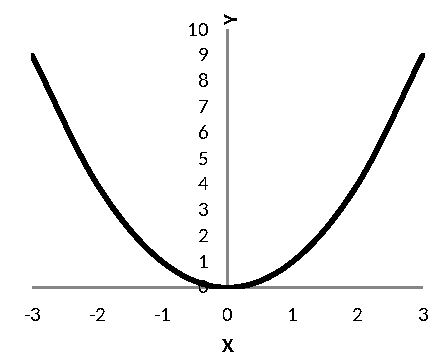
\includegraphics[width=0.45\textwidth]{capitulos/funcao_do_primeiro_grau/media/image28.pdf} 
	d) 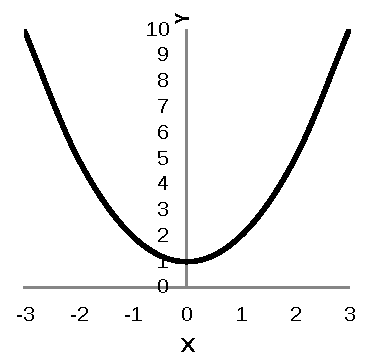
\includegraphics[width=0.45\textwidth]{capitulos/funcao_do_primeiro_grau/media/image29.pdf}
\end{figure}

\begin{figure}[H]
	e) 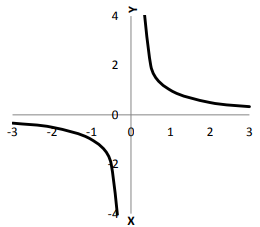
\includegraphics[width=0.45\textwidth]{capitulos/funcao_do_primeiro_grau/media/image30.png} 
	f) 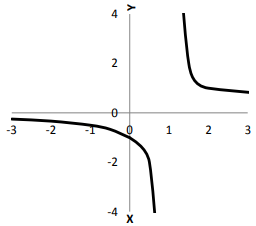
\includegraphics[width=0.45\textwidth]{capitulos/funcao_do_primeiro_grau/media/image31.png}
\end{figure}

\begin{figure}[H]
	\ansitem{}

	a) 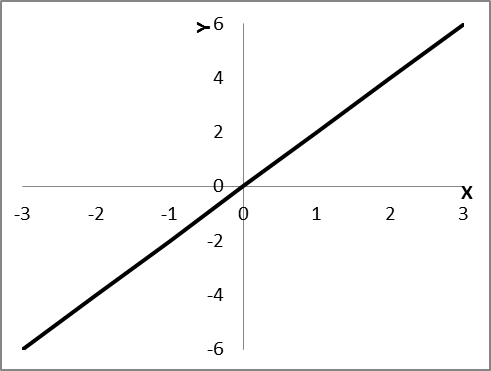
\includegraphics[width=0.45\textwidth]{capitulos/funcao_do_primeiro_grau/media/image32.png} 
	b) 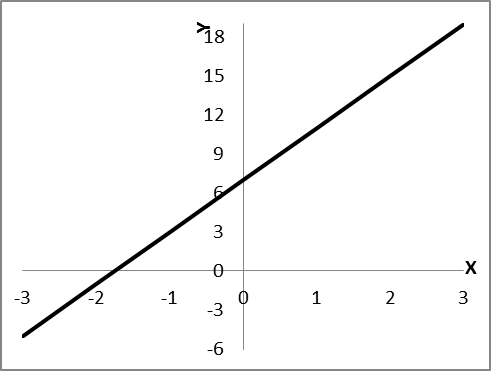
\includegraphics[width=0.45\textwidth]{capitulos/funcao_do_primeiro_grau/media/image33.png}
\end{figure}

\begin{figure}[H]
	c)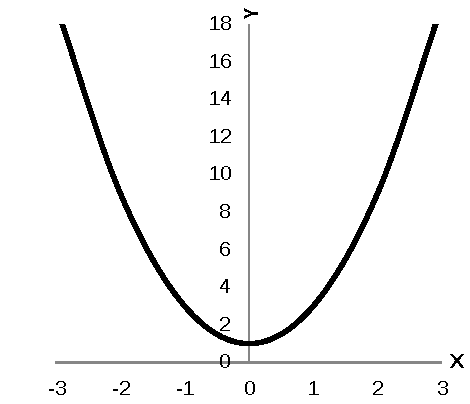
\includegraphics[width=0.45\textwidth]{capitulos/funcao_do_primeiro_grau/media/image34.pdf} 
	d) 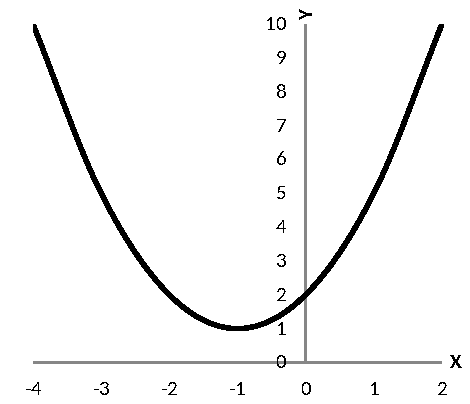
\includegraphics[width=0.45\textwidth]{capitulos/funcao_do_primeiro_grau/media/image35.pdf}
\end{figure}

\ansitem{} Sim.

\ansitem{} Não, pois para um mesmo valor de \textit{x} há dois valores de \textit{y} correspondentes.

\begin{figure}[H]
	\ansitem{}

	a) 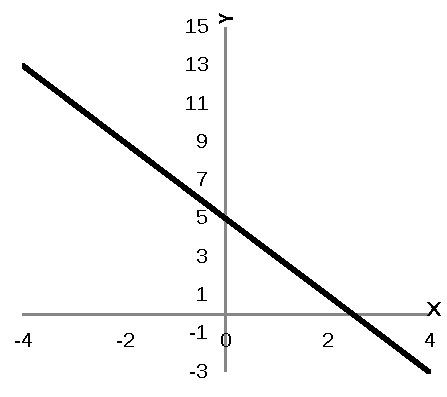
\includegraphics[width=0.45\textwidth]{capitulos/funcao_do_primeiro_grau/media/image36.pdf} 
	b) 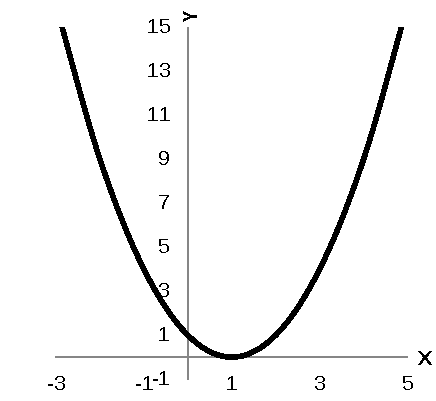
\includegraphics[width=0.45\textwidth]{capitulos/funcao_do_primeiro_grau/media/image37.pdf}
\end{figure}

\begin{figure}[H]
	c) 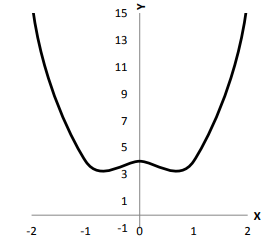
\includegraphics[width=0.45\textwidth]{capitulos/funcao_do_primeiro_grau/media/image38.png} 
	d) 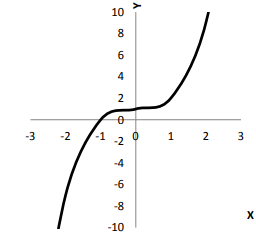
\includegraphics[width=0.45\textwidth]{capitulos/funcao_do_primeiro_grau/media/image39.png}
\end{figure}

\begin{figure}[H]
	e) 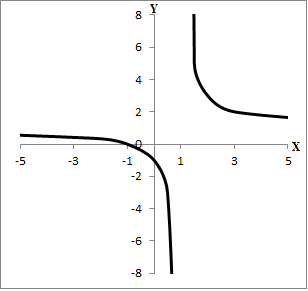
\includegraphics[width=0.45\textwidth]{capitulos/funcao_do_primeiro_grau/media/image40.png} 
	f) 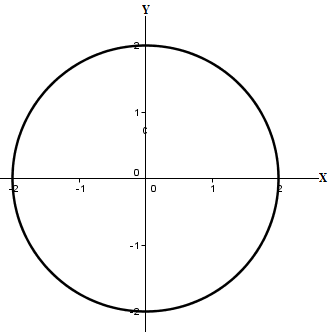
\includegraphics[width=0.45\textwidth]{capitulos/funcao_do_primeiro_grau/media/image41.png}
\end{figure}

\ansitem{} Não, a alternativa f) não está de acordo, pois há dois valores de \textit{y} para mesmo \textit{x.}

\ansitem{} a)  \( D= \left\{ x \in R \right\} ; ~~~ Im= \{ y \in R \}  \)

b)  \( D= \left\{ x \in R \neq 0 \right\} ;~~~~~~ Im= \{ y \in  R / y \neq 1 \}  \) 

c)  \( D= \left\{ x \in R \right\} ; Im= \{ y \in R / y \leq 4 \}  \) 

d)  \( D= \left\{ x \in R/x \geq 0 \right\} ; Im= \{ y \in R/y \geq 0 \}  \) 

e)  \( D= \left\{ x \in R/x \geq 0 \right\} ; Im= \{ y \in R/y \leq 0 \}  \) 

f)  \( D= \left\{ x \in R/x \geq 4 \right\} ; Im= \{ y \in R/y \geq 0 \}  \) 
\end{respostas}

\begin{respostas}{3}
\ansitem{} a) Sim. A dependência é de 1º Grau.

b) A proporção da circunferência em relação ao raio é de 1º Grau. A da área é de 2º Grau.

c) Sim. A dependência é de 1º Grau.

d) Sim. A dependência é de 1º Grau.

e) Sim. A dependência é de 1º Grau.

\ansitem{} \textit{m }é proporcional a \textit{y.  \(  \Delta y/ \Delta x=50/3 \) }

\ansitem{}  \( y \left( x \right) =1,5x+5 \) 

\ansitem{}  \( C \left( x \right) =p \cdot x \) ; 

\ansitem{}  \( C \left( x \right) =px+b \) 

\ansitem{}  \( C \left( x \right) =ax+CF \) 

\ansitem{} a)  \( a=1/2; b= 1/2 \) ;  \( f \left( x \right) =\frac{1}{2}x+\frac{1}{2} \) \tab \tab 

b)  \( a=1; b= 3; \)   \( f \left( x \right) =x+3 \) \tab \tab 

c) \(  a= -1; b= 0; \)   \( f \left( x \right) =-x \) \tab \tab 

d) \(  a= 0; b= 3; f \left( x \right) =3 \) 

\ansitem{} a) C=20/7x +5/7 \qquad b) C(30)=605/7= 86,43

\ansitem{}

\begin{multicols}{2}
a)  \( a=-3; Decrescente \)

b)  \( a=-1/2; Decrescente \) 

c)  \( a= -2/3; Decrescente \)

d) \(  a=1; Crescente \)
\end{multicols}

\ansitem{} a) \( f \left( x \right) =\frac{1}{2}x+1 \)  

\begin{figure}[H]
	\begin{Center}
		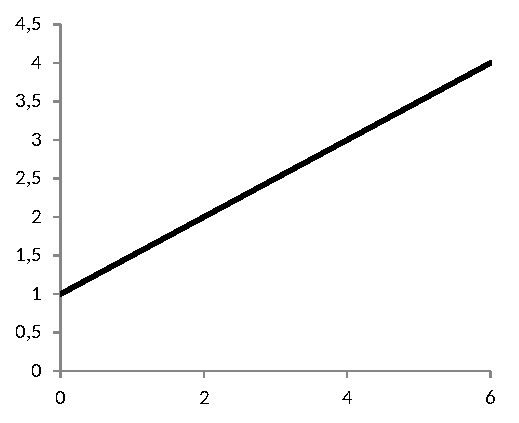
\includegraphics[width=3.07in,height=1.91in]{capitulos/funcao_do_primeiro_grau/media/image42.pdf}
	\end{Center}
\end{figure}

b) Os pontos não estão alinhados

\ansitem{}  \textit{V\textsubscript{1}V\textsubscript{2}:x=0; V\textsubscript{1}V\textsubscript{4}:y=0; V\textsubscript{2}V\textsubscript{3}:y=4; V\textsubscript{3}V\textsubscript{4}:x=4}

\ansitem{}  \textit{V\textsubscript{1}V\textsubscript{2}:y=1; V\textsubscript{1}V\textsubscript{3}:x=1; V\textsubscript{2}V\textsubscript{3}:y=-x+5}

\begin{figure}[H]
	\ansitem{}

	a) 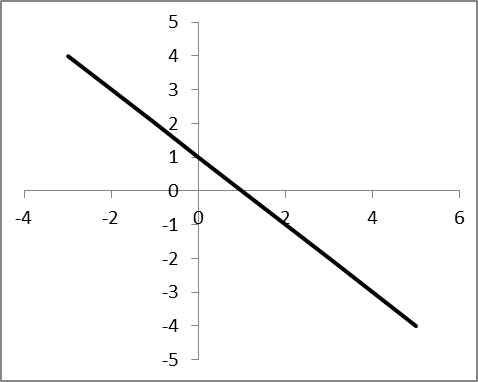
\includegraphics[width=0.45\textwidth]{capitulos/funcao_do_primeiro_grau/media/image43.png} 
	b) 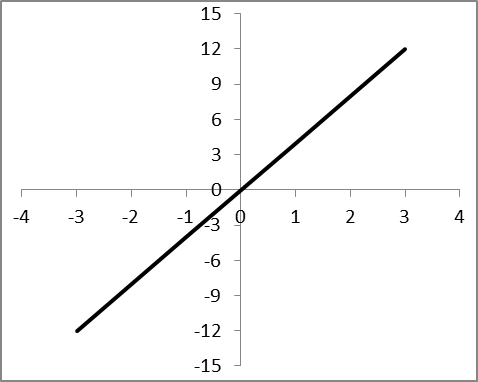
\includegraphics[width=0.45\textwidth]{capitulos/funcao_do_primeiro_grau/media/image44.png}
\end{figure}

\begin{figure}[H]
	c) 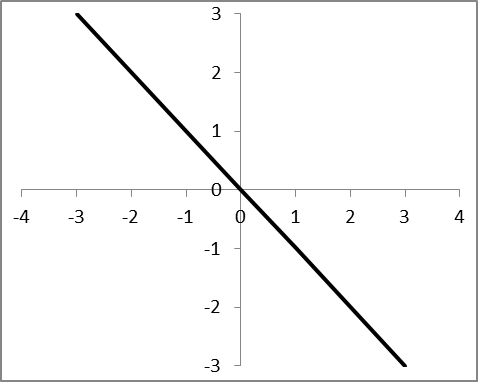
\includegraphics[width=0.45\textwidth]{capitulos/funcao_do_primeiro_grau/media/image45.png} 
	d) 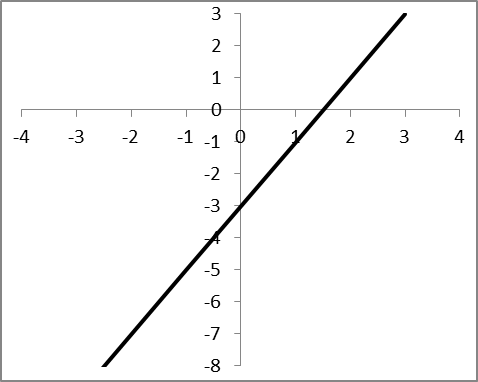
\includegraphics[width=0.45\textwidth]{capitulos/funcao_do_primeiro_grau/media/image46.png}
\end{figure}

\begin{figure}[H]
	e) 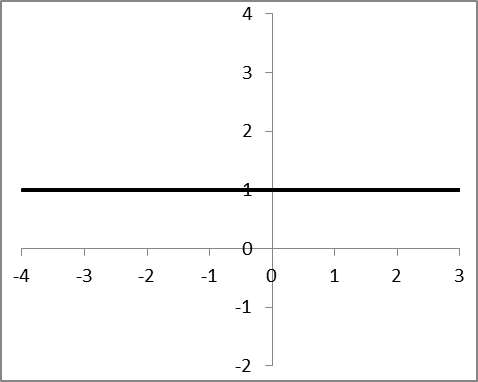
\includegraphics[width=0.45\textwidth]{capitulos/funcao_do_primeiro_grau/media/image47.png} 
	f) 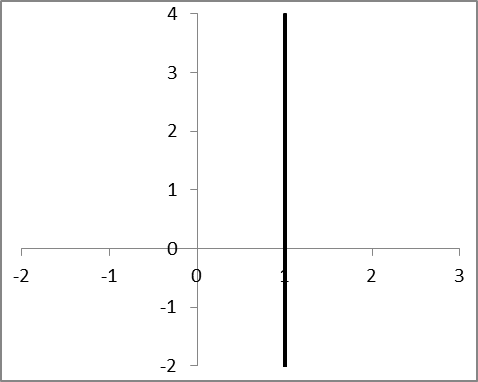
\includegraphics[width=0.45\textwidth]{capitulos/funcao_do_primeiro_grau/media/image48.png}
\end{figure}

\begin{figure}[H]
	\ansitem{}

	a) 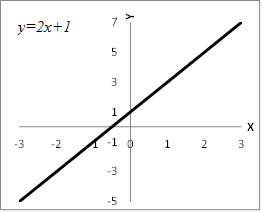
\includegraphics[width=0.45\textwidth]{capitulos/funcao_do_primeiro_grau/media/image49.png} 
	b) 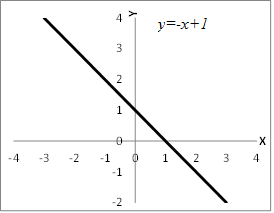
\includegraphics[width=0.45\textwidth]{capitulos/funcao_do_primeiro_grau/media/image50.png}
\end{figure}

\begin{figure}[H]
	c) 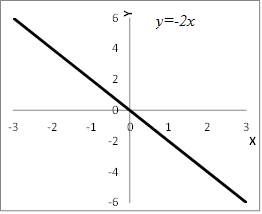
\includegraphics[width=0.45\textwidth]{capitulos/funcao_do_primeiro_grau/media/image51.png} 
	d) \includegraphics[width=0.45\textwidth]{capitulos/funcao_do_primeiro_grau/media/image52.png}
\end{figure}

\begin{figure}[H]
	e) \includegraphics[width=0.45\textwidth]{capitulos/funcao_do_primeiro_grau/media/image53.png} 
	f) \includegraphics[width=0.45\textwidth]{capitulos/funcao_do_primeiro_grau/media/image54.png}
\end{figure}

\ansitem{} a)  \( f \left( x \right) =40x+3 \)  \qquad b)  \( g \left( x \right) =50x+3 \) 

\begin{figure}[H]
	\includegraphics[width=0.45\textwidth]{capitulos/funcao_do_primeiro_grau/media/image55.png} 
	\includegraphics[width=0.45\textwidth]{capitulos/funcao_do_primeiro_grau/media/image56.png}
\end{figure}

\ansitem{} a) Crescente; Intersecção em Y: (0,5) \qquad b) Decrescente; Intersecção em Y: (0,-1)

\begin{figure}[H]
	\includegraphics[width=0.45\textwidth]{capitulos/funcao_do_primeiro_grau/media/image57.pdf} 
	\includegraphics[width=0.45\textwidth]{capitulos/funcao_do_primeiro_grau/media/image58.pdf}
\end{figure}

c) Crescente; Intersecção em Y: (0,-1.3) \qquad d) Decrescente; Intersecção em Y:(0,2.3)

\begin{figure}[H]
	\includegraphics[width=0.45\textwidth]{capitulos/funcao_do_primeiro_grau/media/image59.pdf} 
	\includegraphics[width=0.45\textwidth]{capitulos/funcao_do_primeiro_grau/media/image60.pdf}
\end{figure}

e) Decrescente; Intersecção em Y:(0,2) \qquad f) Decrescente; Intersecção em Y:(0,-5)

\begin{figure}[H]
	\includegraphics[width=0.45\textwidth]{capitulos/funcao_do_primeiro_grau/media/image61.pdf} 
	\includegraphics[width=0.45\textwidth]{capitulos/funcao_do_primeiro_grau/media/image62.pdf}
\end{figure}

\ansitem{} a) Crescente; Ponto de Intersecção em Y= -2

 b) Decrescente; Ponto de Intersecção em Y=27/4

 c) Decrescente; Ponto de Intersecção em Y=54/5

 d) Decrescente; Ponto de Intersecção em Y=17/5

\ansitem{}

\begin{multicols}{2}
\begin{table}[H]
a)

\begin{tabular}{p{0.37in}p{0.39in}}
\hline
%row no:1
\multicolumn{1}{|p{0.37in}}{X} & 
\multicolumn{1}{|p{0.39in}|}{Y} \\
\hhline{--}
%row no:2
\multicolumn{1}{|p{0.37in}}{0} & 
\multicolumn{1}{|p{0.39in}|}{20} \\
\hhline{--}
%row no:3
\multicolumn{1}{|p{0.37in}}{1} & 
\multicolumn{1}{|p{0.39in}|}{170} \\
\hhline{--}
%row no:4
\multicolumn{1}{|p{0.37in}}{5} & 
\multicolumn{1}{|p{0.39in}|}{770} \\
\hhline{--}
%row no:5
\multicolumn{1}{|p{0.37in}}{10} & 
\multicolumn{1}{|p{0.39in}|}{1520} \\
\hhline{--}
%row no:6
\multicolumn{1}{|p{0.37in}}{50} & 
\multicolumn{1}{|p{0.39in}|}{7520} \\
\hhline{--}
\end{tabular}
 \end{table}

\begin{figure}[H]
	b)
	
	\includegraphics[width=2.88in,height=2.24in]{capitulos/funcao_do_primeiro_grau/media/image63.png}
\end{figure}
\end{multicols}

 c)  \( C(x)=150x+20 \) \tab d)150 é o custo de produção de uma peça e 20 \tab é o custo unitário. 

\ansitem{}

\begin{figure}[H]
	a)
	
	\includegraphics[width=2.79in,height=1.8in]{capitulos/funcao_do_primeiro_grau/media/image64.png}
\end{figure}

b) Candidato (A):  \( y=\frac{2}{31}x+\frac{1083}{31} \) , Percentual para 20/07: 36,22$\%$ 

Candidato (B):  \( y=\frac{2}{31}x+\frac{928}{31} \) , Percentual para 20/07: 31,22$\%$ 

c) Candidato (A): 51,8$\%$ 

Candidato (B): 45,1$\%$ 
\end{respostas}

\section{ANEXO}

\subsection{Tangente de ângulos suplementares}

Sejam o ângulo \textit{0 <  < 90º}. O suplementar de   é (\textit{180º - }). Pela definição de tangente,  \( tg \left(  \theta  \right) =MT \)   e  \( tg \left( 180 ^{\circ} - \theta  \right) =MT' \)  , como mostra a Fig. 1. Os ângulos dos triângulos OMT e OMT’ são iguais e o segmento OM é comum aos triângulos (portanto são iguais) então os outros lados também serão. Portanto, os triângulos OMT e OMT’ são idênticos e 

 \[ tg \left(  \theta  \right) =-tg \left( 180 ^{\circ} - \theta  \right)  \] 

\begin{figure}[H]
	\begin{Center}
		\includegraphics[width=3.08in,height=2.64in]{capitulos/funcao_do_primeiro_grau/media/image65.png}
	\end{Center}
\end{figure}

Figura 1 - Tangente de ângulos suplementares

\subsection{Tangente de ângulos complementares}

Pela definição de tangente, temos:

 \( tg \left(  \theta  \right) =\frac{QR}{PR} \)        e     \( tg \left( 90^{o}- \theta  \right) =\frac{PR}{QR} \)   . Comparando as expressões, temos:

 \[ tg \left(  \theta  \right) =\frac{1}{tg \left( 90^{o}- \theta  \right) } \] 

\begin{figure}[H]
	\begin{Center}
		\includegraphics[width=2.35in,height=2.34in]{capitulos/funcao_do_primeiro_grau/media/image66.png}
	\end{Center}
\end{figure}

\begin{Center}
Figura 2 - Tangente de ângulos complementares
\end{Center}

\subsection{Retas paralelas}

\textbf{Teorema}: Sejam as retas    (\textit{r) :}   \textit{y = mx + b}   e   (\textit{s) :}   \textit{y = px + c}    . Se \textit{r} é paralela a \textit{s} então \textit{m = p}.   

\textbf{Demonstração}: Sejam    e    os ângulos que as retas \textit{r} e \textit{s}, fazem com o eixo \textit{X}, respectivamente. Se \textit{r} é paralela a \textit{s} então    =      e\textit{   tg    =  tg }  . Como \textit{m=} \textit{tg   }e \textit{p} = \textit{tg }  , tem-se   \textit{m = p}.

\subsection{Retas perpendiculares}

\textbf{Teorema}: Sejam as retas    (\textit{r) :}   \textit{y = mx + b}   e   (\textit{s) :}   \textit{y = px + c}    . Se \textit{r} é perpendicular a  \textit{s}  então      \( p=-\frac{1}{m} \)   .

\textbf{Demonstração:} Sejam    e    os ângulos que as retas \textit{r} e \textit{s}, fazem com o eixo \textit{X}, respectivamente. Da Fig. 3, temos:

 \( p=tg \left(  \alpha  \right) =\frac{RP}{PT} \)    ;    \( tg \left( 180^{o}- \theta  \right) =\frac{PT}{RP} \)       e    \tab  \( m=tg \left(  \theta  \right)  \) \tab \tab (3.1)

Da trigonometria sabemos que as tangentes de ângulos suplementares são iguais em módulo e de sinais contrários:

\begin{FlushRight}
 \( tg \left( 180 ^{\circ} - \theta  \right)  =-tg \left(  \theta  \right)  \). \tab (3.2)
\end{FlushRight}

Substituindo a Eq. (3.2) na Eq. (3.1), temos:

\begin{FlushRight}
 \( tg \left(  \theta  \right) =-\frac{PT}{RP} \) \tab (3.3)
\end{FlushRight}

Comparando as razões das Eqs. (3.1) e (3.3) temos:

\( p=tg \left(  \alpha  \right) =\frac{RP}{PT}=-\frac{1}{tg \left(  \theta  \right) }=-\frac{1}{m} \)

\begin{figure}[H]
	\begin{Center}
		\includegraphics[width=3.24in,height=2.79in]{capitulos/funcao_do_primeiro_grau/media/image67.png}

		Figura 3 - Retas perpendiculares
	\end{Center}
\end{figure}